\documentclass{beamer}
%\definecolor{envy}{HTML}{1A936F}
%\definecolor{berry}{HTML}{C6878F}
%\colorlet{lberry}{berry!55!white}
%\definecolor{turq}{HTML}{077187}
%\definecolor{pgreen}{HTML}{CBE896}
%\definecolor{db}{HTML}{074F57}
%\colorlet{ldb}{db!55!white}
%\colorlet{lpgreen}{pgreen!55!white}
\definecolor{envy}{HTML}{1A936F}
\definecolor{berry}{HTML}{E3463F}
\colorlet{lberry}{berry!55!white}
\definecolor{turq}{HTML}{077187}
\definecolor{pgreen}{HTML}{FD9564}
\definecolor{db}{HTML}{213862}
\colorlet{ldb}{db!55!white}
\colorlet{lpgreen}{pgreen!55!white}
\newcommand{\light}[1]{\textcolor{db!50!white}{#1}}
% New colours!
% \setbeamercolor{background canvas}{bg=GreyWhite}
\setbeamercolor{title}{fg=db, bg=pgreen!55!white}
\setlength{\intextsep}{-1ex} % remove extra space above and below in-line float
%\setbeamercolor{frametitle}{fg=black, bg=pgreen!55!white}
%\setbeamercolor{normal text}{fg=black}
%\setbeamercolor{block title}{fg=black,bg=pgreen!55!white}
\setbeamercolor{frametitle}{fg=db, bg=pgreen!55!white}
\setbeamercolor{normal text}{fg=db}
\setbeamercolor{block title}{fg=db,bg=pgreen!55!white}
\setbeamercolor{block body}{fg=black!22!white}
%\setbeamercolor{alerted text}{fg=Pinky}
\setbeamercolor{itemize item}{fg=berry}
\setbeamercolor{itemize subitem}{fg=berry}
\setbeamercolor{itemize subsubitem}{fg=berry}
%\setbeamercolor{framesource}{fg=Carrot}
%\setbeamercolor{section in toc}{fg=PurpNav}
\setbeamercolor{footnote}{fg=black}
\setbeamercolor{footnote mark}{fg=black}
\setbeamercolor{myfootlinetext}{fg=black}
\setbeamertemplate{itemize subitem}{fg=berry}
\setbeamertemplate{itemize subsubitem}{fg=berry}
%\setbeamertemplate{itemize item}{\color{DarkPurple}$\blacksquare$}
%\setbeamertemplate{itemize item}{\color{DarkPurple}}[circle]
\setbeamertemplate{itemize item}[circle]

\newcommand{\be}{\begin{enumerate}}
	\newcommand{\ee}{\end{enumerate}}
\newcommand{\bi}{\begin{itemize}}
	\newcommand{\ei}{\end{itemize}}
\newcommand{\ccbb}{\cellcolor{turq!15!white}}
\newcommand{\cc}{\cellcolor{pgreen!55!white}}
\newcommand{\ccb}{\cellcolor{berry!35!white}}

% source at bottom left of slide
\newcommand{\sourceleft}[1]{\begin{textblock*}{4cm}(0.3cm,8.8cm)
		\begin{beamercolorbox}[ht=0.5cm,left]{framesource}
			\usebeamerfont{framesource}\usebeamercolor[fg]{framesource}
			{#1}
		\end{beamercolorbox}
	\end{textblock*}}
	
% source at bottom right of slide
\newcommand{\sourceright}[1]{\begin{textblock*}{}
		\begin{beamercolorbox}[ht=0.5cm,left]{framesource}
			\usebeamerfont{framesource}\usebeamercolor[berry]{framesource}
			{#1}
		\end{beamercolorbox}
	\end{textblock*}}

\newcommand{\cfcite}[1]{\footnote{\citeauthor{#1}, \citeyear{#1}}}

\newcommand{\sourceextremeright}[1]{\begin{textblock*}{4cm}(10.6cm,8.8cm)
		\begin{beamercolorbox}[ht=0.5cm,left]{framesource}
			\usebeamerfont{framesource}\usebeamercolor[fg]{framesource}
			{#1}
		\end{beamercolorbox}
	\end{textblock*}}

\usetheme{boxes}
\usepackage[absolute,overlay]{textpos}
%\usecolortheme{beaver}
\useinnertheme{circles}
\usepackage{amsmath}
\usepackage{amssymb}
\usepackage{lmodern}
\usepackage{xcolor}
\usepackage{tikz-cd}
\usepackage{tikz}
\usetikzlibrary{decorations.markings}
\usetikzlibrary{calc, arrows}
\usepackage{longtable}
\usepackage{graphicx}% http://ctan.org/pkg/graphicx
\usepackage{booktabs}
\usepackage{xspace}
\usepackage{varwidth}
\usepackage{array} %make columns all same width
\newcolumntype{C}{>{\centering\arraybackslash}p{0.2\linewidth}}
\usepackage{scrtime} % for \thistime (this package MUST be listed first!)
\usepackage{amsmath} % essential for cases environment
\usepackage{amsthm} % for theorems and proofs
\usepackage{amsfonts} % mathbb
\usepackage{graphics,graphicx}
\usepackage{multirow} % fancy tables
\usepackage{wasysym} % circle symbols (including half-filled circles)
\usepackage{enumerate} % fancier enumeration (e.g., a,b,c, ...)
%\usepackage{xcolor}
\usepackage{color}
\usepackage{xstring}
\usepackage[misc]{ifsym} %for email mail symbol
\usepackage[linguistics]{forest}
\usetikzlibrary{calc, arrows}
\usepackage{xcolor,colortbl}
\usepackage[export]{adjustbox}
%\colorlet{grey}{black!10}
%below adds slide number without putting total number of slides
\setbeamertemplate{footline}{%
	\raisebox{5pt}{\makebox[\paperwidth]{\hfill\makebox[10pt]{\scriptsize\insertframenumber}}}}

\newenvironment{itmenv}{\only{\setbeamercolor{local structure}{fg=gray}}}{}
\setbeamertemplate{enumerate items}[default]
\setbeamercolor*{enumerate item}{fg=db}

\setbeamercolor*{enumerate subitem}{fg=db}

\newcommand\FrameText[1]{%
	\begin{textblock*}{\paperwidth}(0pt,\textheight)
		\raggedleft #1\hspace{4em}\vspace{20em}
	\end{textblock*}}

\mode<presentation>
\title{\Huge Bioinformatics: \\ the hot interdisciplinary field}

\author[Daniella Lato]{\\ \textbf{Daniella Lato}\\ (She/Her) \\ PhD Candidate \\ Biology Department \\ Golding Lab, McMaster}
\date[2019]{\Letter \xspace latodf@mcmaster.ca \\ \texttt{GitHub}: \url{https://github.com/dlato}}
\IfFileExists{upquote.sty}{\usepackage{upquote}}{}
\newcommand{\itm}{\item<itm@1->}
\newcommand{\btVFill}{\vskip0pt plus 1filll}
\newcommand{\s}{\textit{Sinorhizobium}\ }
\newcommand{\sm}{\textit{Sinorhizobium meliloti}\xspace}
\newcommand{\salm}{\textit{Salmonella enterica}\xspace}
\newcommand{\smel}{\textit{S.\,meliloti}\xspace}
\newcommand{\smed}{\textit{S.\,medicae}}
\newcommand{\sfred}{\textit{S.\,fredii}}
\newcommand{\ssah}{\textit{S.\,saheli}}
\newcommand{\ster}{\textit{S.\,terangae}}
\newcommand{\ag}{\textit{Agrobacterium tumefaciens }}
\newcommand{\p}{progressiveMauve\xspace}
\newcommand{\agro}{\textit{A.\,tumefaciens }}
\newcommand{\bur}{\textit{Burkholderia}\xspace}
\newcommand{\vib}{\textit{Vibrio}\xspace}
\newcommand{\bor}{\textit{Bordetella}\xspace}
\newcommand{\xan}{\textit{Xanthomonas}\xspace}
\newcommand{\sul}{\textit{Sulfolobus}\xspace}
\newcommand{\ent}{\textit{Enterobacteria}\xspace}
\newcommand{\bac}{\textit{Bacillus subtilis}\xspace}
\newcommand{\ecoli}{\textit{Escherichia coli}\xspace}
\newcommand{\lis}{\textit{Listeria monocytogenes}\xspace}
\newcommand{\bass}{\textit{B.\,subtilis}\xspace}
\newcommand{\bas}{\textit{Bacillus subtilis}\xspace}
\newcommand{\tub}{\textit{Mycobacterium tuberculosis}\xspace}
\newcommand{\strep}{\textit{Streptomyces}\xspace}
\newcommand{\agrot}{\textit{Agrobacterium tumefaciens}\xspace}
\newcommand{\ecol}{\textit{E.\,coli}\xspace}
\newcommand{\salb}{\textit{S.\,alblus}\xspace}
\newcommand{\salbus}{\textit{S.\,albus}\xspace}
\newcommand{\shyg}{\textit{S.\,hygroscopicus}\xspace}
\newcommand{\sliv}{\textit{S.\,lividans}\xspace}
\newcommand{\sros}{\textit{S.\,roseosporus}\xspace}
\newcommand{\ssir}{\textit{S.\,sirex}\xspace}
\newcommand{\sven}{\textit{S.\,venezuelae}\xspace}
\newcommand{\scoe}{\textit{S.\,coelicolor}\xspace}
\newcommand{\hal}{\textit{Haloquadratum walsbyi}\xspace}
\newcommand{\pa}{pSymA\xspace}
\newcommand{\pb}{pSymB\xspace}
\newcommand{\dn}{\textit{dN}\xspace}
\newcommand{\ds}{\textit{dS}\xspace}
\newcommand{\rhod}{\textit{Rhodobacteraceae}\xspace}
\newcommand{\burcen}{\textit{Burkholderia cenocepacia}\xspace}
\setbeamertemplate{navigation symbols}{}
\newcommand*{\NodeSize}{0.5cm}%
\newcommand*{\YShiftBetweenRows}{-1cm}% Subsequent rows are shited down so they don't overlap
\tikzset{DNA Style/.style={minimum size=0.5cm, draw=gray, line width=1pt}}{}
\providecommand{\e}[1]{\ensuremath{\times 10^{#1}}}
\newlength{\YShift}% 
\newcounter{ColumnCounter}% Prefix for node 
%anestral recon fig colours
\colorlet{darkcol}{lberry}
\colorlet{lightcol}{lpgreen}
\definecolor{txtcol}{HTML}{F2545B}
%\colorlet{txtcol}{pgreen}
% BLACK AND WHITE
%\colorlet{darkcol}{black!30!white}
%\colorlet{lightcol}{black!10!white}
%\definecolor{txtcol}{HTML}{F40000}

\newcommand\FourQuad[4]{%
	\begin{minipage}[b][.35\textheight][t]{.47\textwidth}#1\end{minipage}\hfill%
	\begin{minipage}[b][.35\textheight][t]{.47\textwidth}#2\end{minipage}\\[0.5em]
	\begin{minipage}[b][.35\textheight][t]{.47\textwidth}#3\end{minipage}\hfill
	\begin{minipage}[b][.35\textheight][t]{.47\textwidth}#4\end{minipage}%
}

\usepackage{graphicx}

\usepackage{ragged2e}
\usepackage{xcolor}

\usepackage[most]{tcolorbox}

%below makes a transparent text box
\newtcolorbox{mytransparentbox}[1][]{%
	coltext=db,
	arc=0pt,
	auto outer arc,
	enhanced jigsaw,
	opacityback=0.9,
	%opacityframe=0.0,
	colback=pgreen!55!white,
	width=0cm,
	boxrule=0pt,
	oversize=1cm,
	#1
}

\newenvironment<>{varblock}[2][\textwidth]{%
	\setlength{\textwidth}{#1}
	\begin{actionenv}#3%
		\def\insertblocktitle{#2}%
		\par%
		\usebeamertemplate{block begin}}
	{\par%
		\usebeamertemplate{block end}%
\end{actionenv}}

% Initialize - These are probably not needed, but prefer to set them
\setlength{\YShift}{0cm}% 
\setcounter{ColumnCounter}{0}


%%%%%%%%%%%%%%%%%%%%%%%%%%%%%%%%%%%%%%%%%%%%%%%%%%%%%%%%%%%%%%%%
%%%%%%%%%%%%%%%%%%%%%%%%%%%%%%%%%%%%%%%%%%%%%%%%%%%%%%%%%%%%%%%%%%%%%%%%%%%%%%%%%%%%%%%%%%%%%%%%


\begin{document}
% \titlegraphic{text} %for including logos in title. have to adjust vspace and hspace	
	\begin{frame}
		\titlepage
		
	\end{frame}
	%\begin{frame}
	%\begin{center}
	
	%\huge{Introduction}
	
	%\end{center}
	%\end{frame}

%%%%%%%%%%%%%%%%%%%%%%%%%%%%%%%%%%%%%%%%%%%%%%%
{
	\usebackgroundtemplate{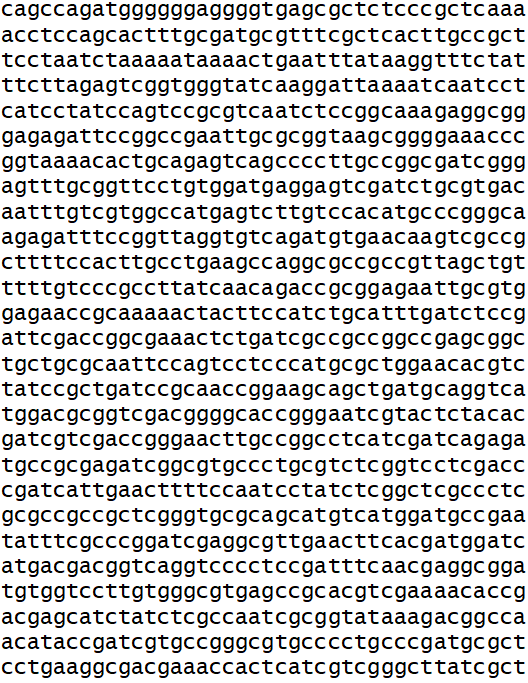
\includegraphics[width=\paperwidth]{./smel_dna.png}}
	\begin{frame}[noframenumbering,plain]{}
		
	\end{frame}
}
%%%%%%%%%%%%%%%%%%%%%%%%%%%%%%%%%%%%%%%%%%%%%%%%%%%%%%
%%%%%%%%%%%%%%%%%%%%%%%%%%%%%%%%%%%%%%%%%%%%%%%%%%%%%%
\begin{frame}{}
\centering
\bigskip
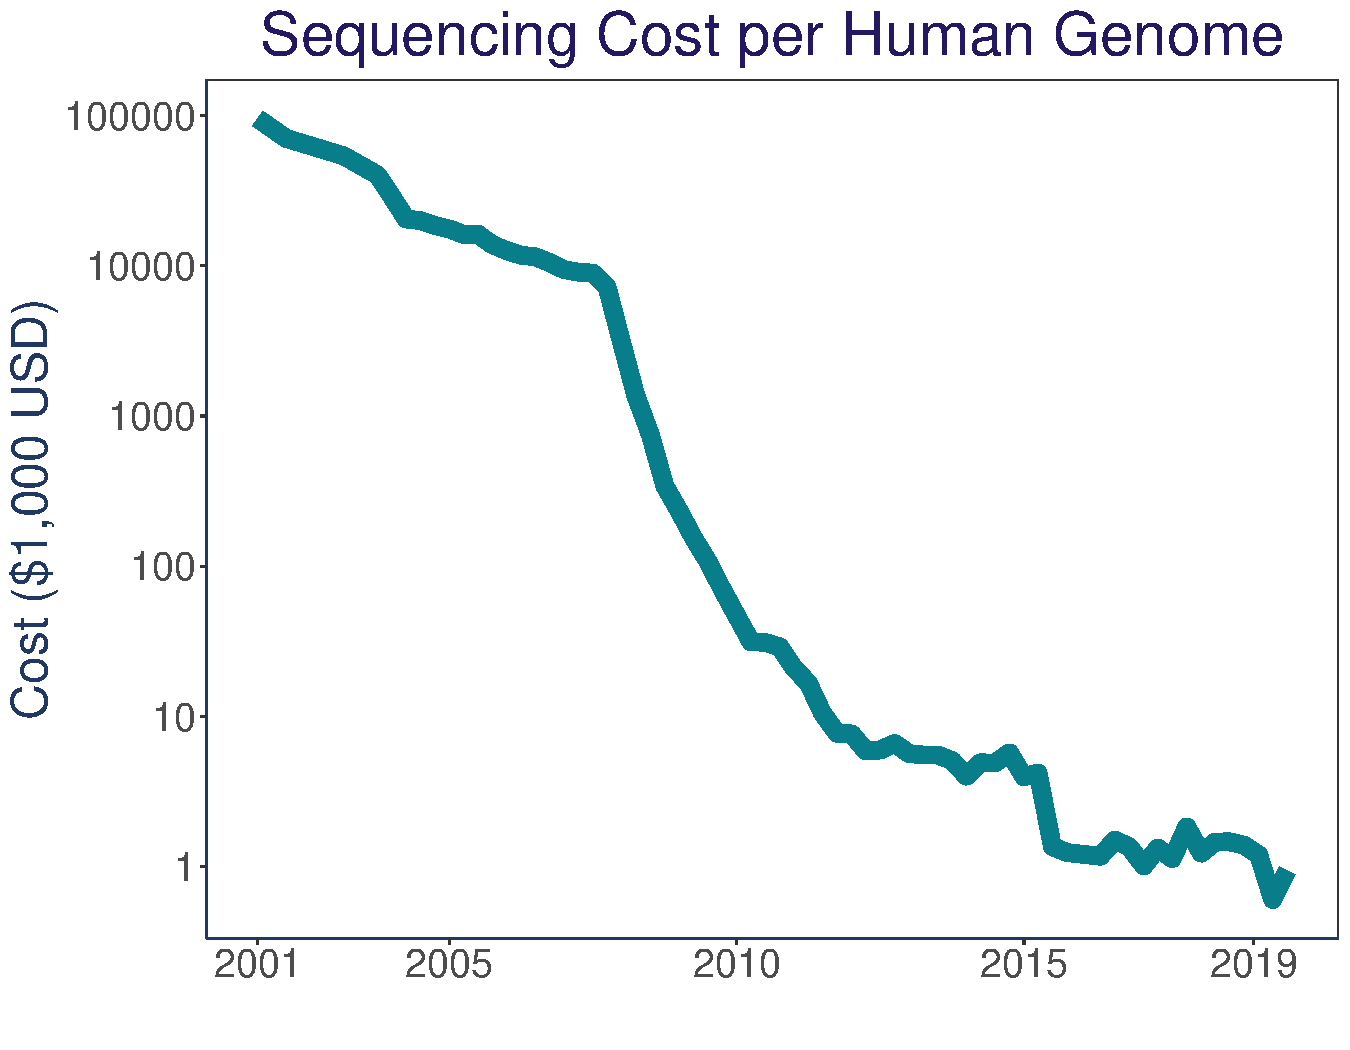
\includegraphics[width=\textwidth]{./seq_cost_graph.pdf}
	\btVFill
		\tiny \vspace{-\baselineskip}\color{berry}{adapted from: Kris Wetterstrand, National Human Genome Research Institute}
\end{frame}
%%%%%%%%%%%%%%%%%%%%%%%%%%%%%%%%%%%%%%%%%%%%%%%%%%%%%%%
%%%%%%%%%%%%%%%%%%%%%%%%%%%%%%%%%%%%%%%%%%%%%%%%%%%%%%%
\begin{frame}{Cost to Sequence a Human Genome in 2019}
	\centering
%	\bigskip
	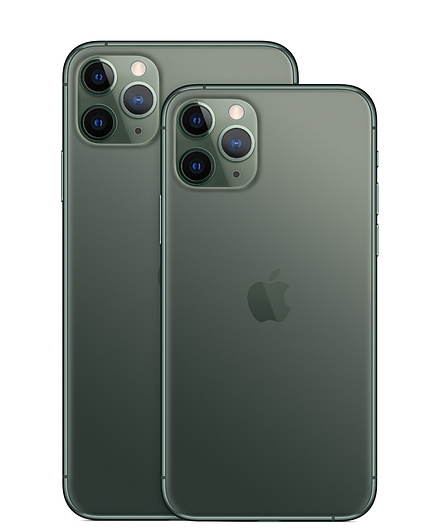
\includegraphics[width=0.5\textwidth]{./iphone.jpg}
	
\end{frame}
%%%%%%%%%%%%%%%%%%%%%%%%%%%%%%%%%%%%%%%%%%%%%%%%%%%%%%
\begin{frame}{}
	\centering
	\bigskip
	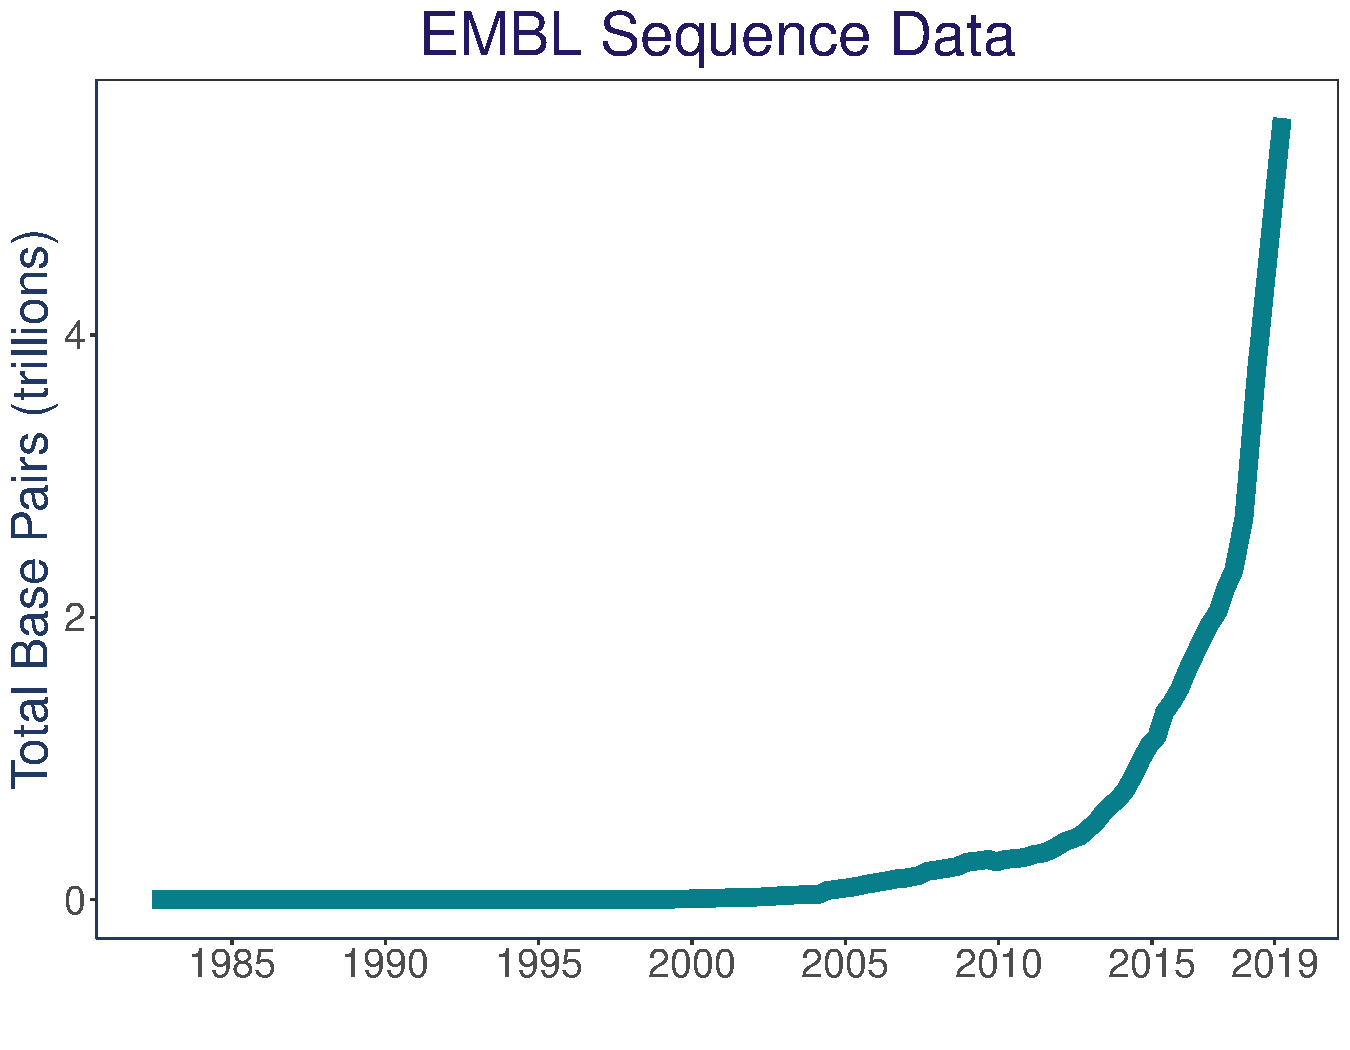
\includegraphics[width=\textwidth]{./seq_num_graph.pdf}
	\btVFill
	\tiny \vspace{-\baselineskip}\color{berry}{Data from: European Molecular Biology Laboratory (EMBL), publicaly available}
%	\textbf{which means that biological data has increased, insert seq number graph here}
	
\end{frame}
%%%%%%%%%%%%%%%%%%%%%%%%%%%%%%%%%%%%%%%%%%%%%%%%%%%%%%
%%%%%%%%%%%%%%%%%%%%%%%%%%%%%%%%%%%%%%%%%%%%%%%%%%%%%%%
\begin{frame}{How many GB is that?}
	
	\centering
		All that sequence data would equal about 
		
		\bigskip

		{\Huge \textbf{11,066,077,343,692 GB}}
	
\end{frame}
%%%%%%%%%%%%%%%%%%%%%%%%%%%%%%%%%%%%%%%%%%%%%%%%%%%%%%
%%%%%%%%%%%%%%%%%%%%%%%%%%%%%%%%%%%%%%%%%%%%%%%%%%%%%%%
\begin{frame}{How many GB is that?}
\begin{minipage}{0.51\textwidth}
	\centering

\includegraphics[width=0.6\textwidth]{./laptop.pdf}
\end{minipage}
\begin{minipage}{0.47\textwidth}
	\Huge
						\textbf{$\approx$ 512GB}
\end{minipage}
\end{frame}
%%%%%%%%%%%%%%%%%%%%%%%%%%%%%%%%%%%%%%%%%%%%%%%%%%%%%%
{
	\usebackgroundtemplate{
\includegraphics[width=\paperwidth]{./many_laptops.png}}
	\begin{frame}[noframenumbering,plain]{}
		\centering
		\begin{textblock}{}(1.7,6.8)%
\begin{varblock}[10.1cm]{\Huge\textbf{22 BILLION LAPTOPS}}
\end{varblock}
\end{textblock}
%		\begin{mytransparentbox}[height=12cm]
%				\centering
%		\Huge\textbf{22 TRILLION LAPTOPS}
%		\end{mytransparentbox}
%%		\textbf{\textcolor{black}{22 TRILLION LAPTOPS}}
	\end{frame}
}


%%%%%%%%%%%%%%%%%%%%%%%%%%%%%%%%%%%%%%%%%%%%%%%
{
	\usebackgroundtemplate{
\includegraphics[width=\paperwidth]{./bioinformatics.jpg}}
	\begin{frame}[noframenumbering,plain]{Bioinformatics to the rescue!}
		
	\end{frame}
}
%%%%%%%%%%%%%%%%%%%%%%%%%%%%%%%%%%%%%%%%%%%%%%%%%%%%%%
%%%%%%%%%%%%%%%%%%%%%%%%%%%%%%%%%%%%%%%%%%%%%%%
\begin{frame}{What is Bioinformatics?}
	\centering
	\Large
	Bioinformatics is taking \textbf{biological data, processes and theories} and \textbf{applying} ``informatics'' techniques (derived from disciplines like \textbf{math, computer science, and statistics}) to understand, organize, and predict biological processes.
	
\end{frame}
%%%%%%%%%%%%%%%%%%%%%%%%%%%%%%%%%%%%%%%%%%%%%%%%%%%%%%
%%%%%%%%%%%%%%%%%%%%%%%%%%%%%%%%%%%%%%%%%%%%%%%
\begin{frame}{Broad Types of Bioinformatics}
	\centering
	\Huge
	\begin{enumerate}
		\item Data Analysis
		\item Software Development
		\item Modeling
	%	\item Combination
	\end{enumerate}
	
\end{frame}
%%%%%%%%%%%%%%%%%%%%%%%%%%%%%%%%%%%%%%%%%%%%%%%%%%%%%%
%%%%%%%%%%%%%%%%%%%%%%%%%%%%%%%%%%%%%%%%%%%%%%%
\begin{frame}{Broad Types of Bioinformatics}
	\centering
	\Huge
	\begin{enumerate}
		\item Data Analysis
		\light{\item Software Development
		\item Modeling}
	%	\item Combination}
	\end{enumerate}
	
\end{frame}
%%%%%%%%%%%%%%%%%%%%%%%%%%%%%%%%%%%%%%%%%%%%%%%%%%%%%%
%%%%%%%%%%%%%%%%%%%%%%%%%%%%%%%%%%%%%%%%%%%%%%%
\begin{frame}{1. Data Analysis}
	\Huge
	\centering
	\textbf{Generating, interpreting, and explaining any biological data}

\end{frame}
%%%%%%%%%%%%%%%%%%%%%%%%%%%%%%%%%%%%%%%%%%%%%%%%%%%%%%
%%%%%%%%%%%%%%%%%%%%%%%%%%%%%%%%%%%%%%%%%%%%%%%
%\begin{frame}{1. Data Analysis}
%	Building the Human Genome
%	\begin{center}
%		%\bigskip
%		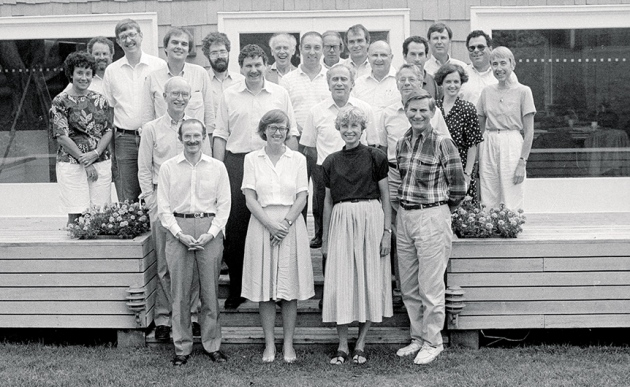
\includegraphics[width=0.97\textwidth]{./HGP_ppl.jpg}
%		
%	\end{center}
%	\btVFill
%	\tiny \vspace{-\baselineskip}\color{berry}{1989: The Banbury meeting at Cold Spring Harbor Laboratory in New York before the launch of the Human Genome Project.}	
%\end{frame}
%%%%%%%%%%%%%%%%%%%%%%%%%%%%%%%%%%%%%%%%%%%%%%%%%%%%%%
%%%%%%%%%%%%%%%%%%%%%%%%%%%%%%%%%%%%%%%%%%%%%%%%%%%%%%
%%%%%%%%%%%%%%%%%%%%%%%%%%%%%%%%%%%%%%%%%%%%%%%
%\begin{frame}{1. Data Analysis}
%	\bigskip
%	\centering
%	
%	\bigskip
%	
%	{\Huge	\textbf{The Human Genome is Sequenced!}}
%	
%	\bigskip
%	
%	International Human Genome Sequencing Consortium Announces ``Working Draft'' of Human Genome, June 2000
%
%
%%	\btVFill
%%	\tiny \vspace{-\baselineskip}\color{berry}{International Human Genome Sequencing Consortium Announces "Working Draft" of Human Genome, June 2000}
%\end{frame}
%%%%%%%%%%%%%%%%%%%%%%%%%%%%%%%%%%%%%%%%%%%%%%%%%%%%%%
%%%%%%%%%%%%%%%%%%%%%%%%%%%%%%%%%%%%%%%%%%%%%%%
\begin{frame}{1. Data Analysis}
	The Human Genome is Sequenced!
	\begin{center}
	%\bigskip
	
\includegraphics[width=0.9\textwidth]{./hgp_covers.png}
\end{center}
	\btVFill
\tiny \vspace{-\baselineskip}\color{berry}{February 2001}
\end{frame}
%%%%%%%%%%%%%%%%%%%%%%%%%%%%%%%%%%%%%%%%%%%%%%%%%%%%%%
%%%%%%%%%%%%%%%%%%%%%%%%%%%%%%%%%%%%%%%%%%%%%%%
\begin{frame}{1. Data Analysis}
	
	{\Large \textbf{1000}} Human Genomes are Sequenced!
	\begin{center}
		%\bigskip
		\includegraphics[width=0.9\textwidth]{./figs/1000Genomes.jpg}
	\end{center}
	\btVFill
	\tiny \vspace{-\baselineskip}\color{berry}{October 2015}
\end{frame}
%%%%%%%%%%%%%%%%%%%%%%%%%%%%%%%%%%%%%%%%%%%%%%%%%%%%%%
%%%%%%%%%%%%%%%%%%%%%%%%%%%%%%%%%%%%%%%%%%%%%%%
%\begin{frame}{1. Data Analysis}
%	The Human Genome is Sequenced...yet AGAIN!
%	\pause
%	\begin{center}
%		\Huge
%		\bigskip
%	\textbf{The complete Human Genome is announced by NHGRI}
%	\end{center}
%	\btVFill
%	\tiny \vspace{-\baselineskip}\color{berry}{National Human Genome Research Institute, April 2003}
%\end{frame}
%%%%%%%%%%%%%%%%%%%%%%%%%%%%%%%%%%%%%%%%%%%%%%%%%%%%%%
%%%%%%%%%%%%%%%%%%%%%%%%%%%%%%%%%%%%%%%%%%%%%%%
%\begin{frame}{1. Data Analysis}
%	\begin{center}
%		\Huge
%		\bigskip
%		\textbf{But is the human genome really ``Complete''?}
%	\end{center}
%
%\end{frame}
%%%%%%%%%%%%%%%%%%%%%%%%%%%%%%%%%%%%%%%%%%%%%%%%%%%%%%
%%%%%%%%%%%%%%%%%%%%%%%%%%%%%%%%%%%%%%%%%%%%%%%
\begin{frame}{Broad Types of Bioinformatics}
	\centering
	\Huge
	\begin{enumerate}
		\item \light{Data Analysis}
		\item Software Development
		\light{	\item Modeling}
	%		\item Combination}
	\end{enumerate}
	
\end{frame}
%%%%%%%%%%%%%%%%%%%%%%%%%%%%%%%%%%%%%%%%%%%%%%%%%%%%%%
%%%%%%%%%%%%%%%%%%%%%%%%%%%%%%%%%%%%%%%%%%%%%%%
\begin{frame}{2. Software Development}
	\centering
	\Huge
	\textbf{Creating bioinformatics tools for other people to use}
	
\end{frame}
%%%%%%%%%%%%%%%%%%%%%%%%%%%%%%%%%%%%%%%%%%%%%%%%%%%%%%
%%%%%%%%%%%%%%%%%%%%%%%%%%%%%%%%%%%%%%%%%%%%%%%
\begin{frame}{2. Software Development}
	\texttt{\p}: Whole genome alignment program
	\pause
	\begin{center}
		%\bigskip
		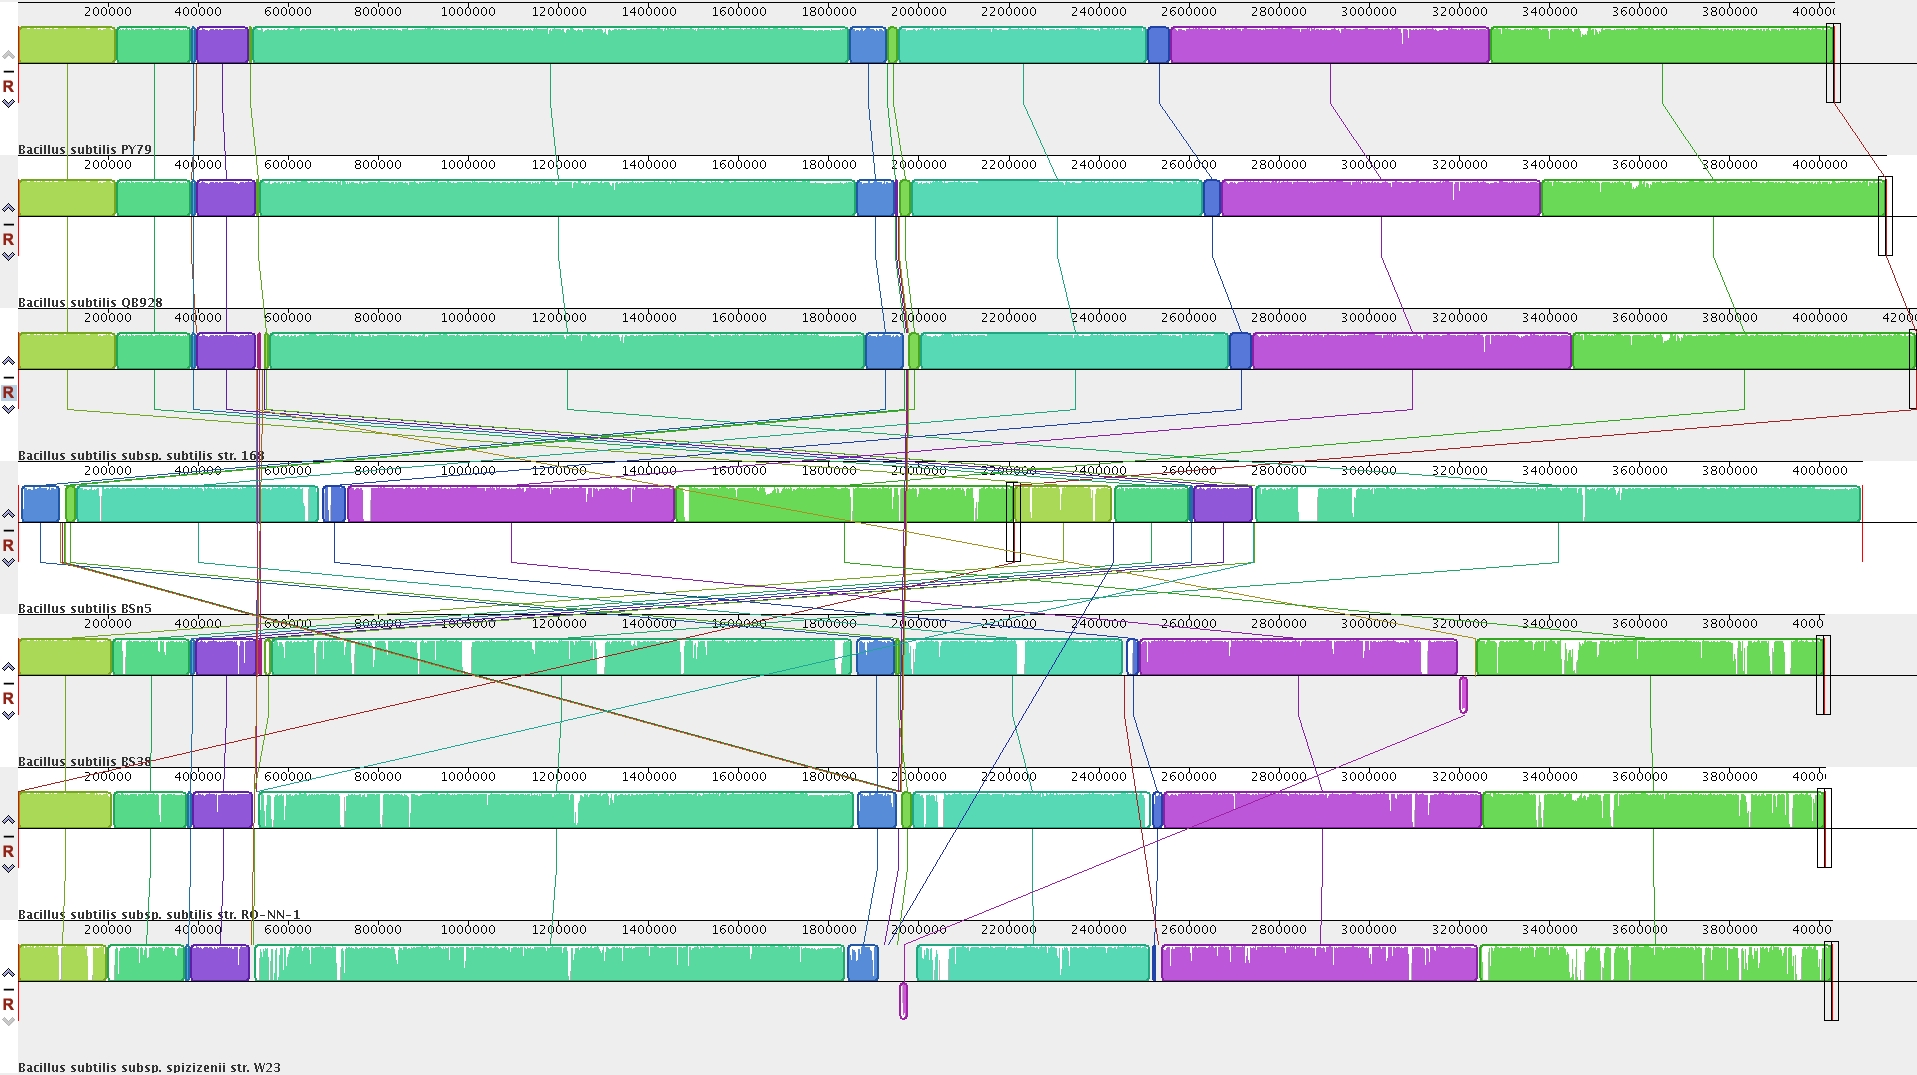
\includegraphics[width=\textwidth]{./Bacillus_alignment_mauve.jpg}
	\end{center}
\btVFill
\tiny \vspace{-\baselineskip}\color{berry}{Darling et al. 2010}
\end{frame}
%%%%%%%%%%%%%%%%%%%%%%%%%%%%%%%%%%%%%%%%%%%%%%%%%%%%%%
%%%%%%%%%%%%%%%%%%%%%%%%%%%%%%%%%%%%%%%%%%%%%%%
\begin{frame}{2. Software Development}
	\texttt{\p}: Whole genome alignment program
	\begin{center}
	%\bigskip
	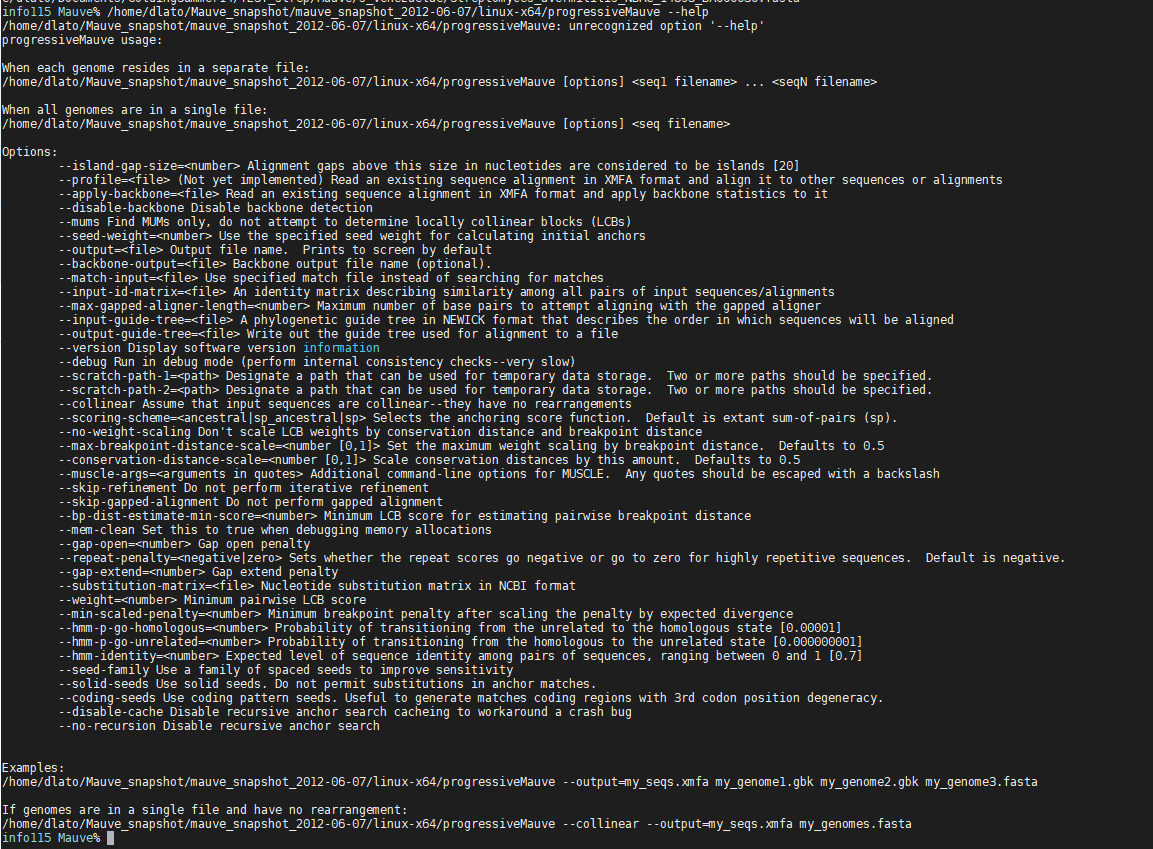
\includegraphics[width=0.85\textwidth]{./linux_mauve.png}
\end{center}
\btVFill
\tiny \vspace{-\baselineskip}\color{berry}{Darling et al. 2010}
\end{frame}
%%%%%%%%%%%%%%%%%%%%%%%%%%%%%%%%%%%%%%%%%%%%%%%%%%%%%%
%%%%%%%%%%%%%%%%%%%%%%%%%%%%%%%%%%%%%%%%%%%%%%%
\begin{frame}{Broad Types of Bioinformatics}
	\centering
	\Huge
	\begin{enumerate}
		\item \light{Data Analysis
		\item Software Development}
		\item Modeling
	%	\light{	\item Combination}
	\end{enumerate}
	
\end{frame}
%%%%%%%%%%%%%%%%%%%%%%%%%%%%%%%%%%%%%%%%%%%%%%%%%%%%%%
%%%%%%%%%%%%%%%%%%%%%%%%%%%%%%%%%%%%%%%%%%%%%%%
\begin{frame}{3. Modelling}
	\Huge
	\centering
	\textbf{Using mathematical and statistical principals to represent and predict biological systems or data}
%Modelling biological systems is a significant task of systems biology and mathematical biology.[a] Computational systems biology[b][1] aims to develop and use efficient algorithms, data structures, visualization and communication tools with the goal of computer modelling of biological systems. It involves the use of computer simulations of biological systems, including cellular subsystems (such as the networks of metabolites and enzymes which comprise metabolism, signal transduction pathways and gene regulatory networks), to both analyze and visualize the complex connections of these cellular processes.[2]	
\end{frame}
%%%%%%%%%%%%%%%%%%%%%%%%%%%%%%%%%%%%%%%%%%%%%%%%%%%%%%
%%%%%%%%%%%%%%%%%%%%%%%%%%%%%%%%%%%%%%%%%%%%%%%
\begin{frame}{3. Modelling}
	SIR model and the Great Plague of London
\begin{center}
	%\bigskip
	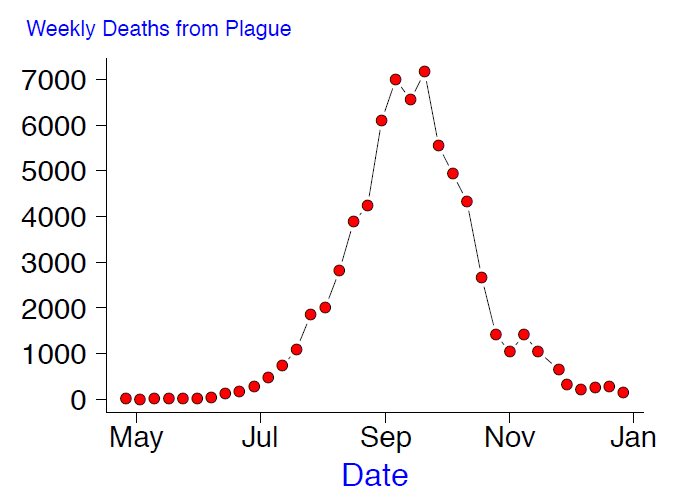
\includegraphics[width=0.93\textwidth]{./figs/plague_no_model.png}
\end{center}
\btVFill
\tiny \vspace{-\baselineskip}\color{berry}{David Earn, McMaster University}
	%Biological systems involve intricate interactions on many spatial and temporal scales. Mathematical models often make it possible to identify mechanisms behind complex biological processes and to predict the outcomes of environmental changes. My current research can be classified according to the time scale over which biological changes occur. Short time scales: Population dynamics of ecological and epidemiological systems. This work, which has implications for conservation of endangered species and eradication of infectious diseases, makes use of modern bifurcation theory. Analytical investigations of discrete maps and differential equations are usually supplemented by extensive numerical studies. Long time scales: Evolutionary dynamics of behavioural traits. This work, which is mainly based on game theoretical analysis, clarifies the adaptive significance of animal behaviour, ranging from cooperation and parental care to foraging and cannabilism.
\end{frame}
%%%%%%%%%%%%%%%%%%%%%%%%%%%%%%%%%%%%%%%%%%%%%%%%%%%%%%
%%%%%%%%%%%%%%%%%%%%%%%%%%%%%%%%%%%%%%%%%%%%%%%
\begin{frame}{3. Modelling}
	SIR model and the Great Plague of London
	\begin{center}
		%\bigskip
		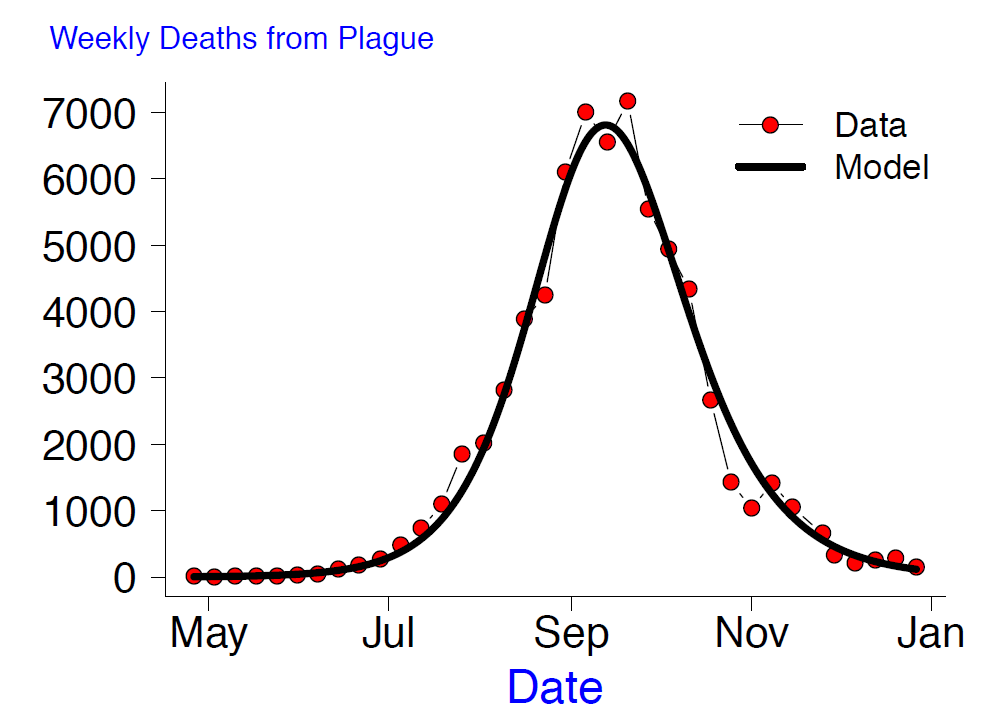
\includegraphics[width=0.95\textwidth]{./modeling_plague.png}
	\end{center}
\btVFill
\tiny \vspace{-\baselineskip}\color{berry}{David Earn, McMaster University}
%Biological systems involve intricate interactions on many spatial and temporal scales. Mathematical models often make it possible to identify mechanisms behind complex biological processes and to predict the outcomes of environmental changes. My current research can be classified according to the time scale over which biological changes occur. Short time scales: Population dynamics of ecological and epidemiological systems. This work, which has implications for conservation of endangered species and eradication of infectious diseases, makes use of modern bifurcation theory. Analytical investigations of discrete maps and differential equations are usually supplemented by extensive numerical studies. Long time scales: Evolutionary dynamics of behavioural traits. This work, which is mainly based on game theoretical analysis, clarifies the adaptive significance of animal behaviour, ranging from cooperation and parental care to foraging and cannabilism.
\end{frame}
%%%%%%%%%%%%%%%%%%%%%%%%%%%%%%%%%%%%%%%%%%%%%%%%%%%%%%
%%%%%%%%%%%%%%%%%%%%%%%%%%%%%%%%%%%%%%%%%%%%%%%
\begin{frame}{3. Modelling}
	Bifurcation theory and predator-prey relationships
	\begin{center}
	%\bigskip
	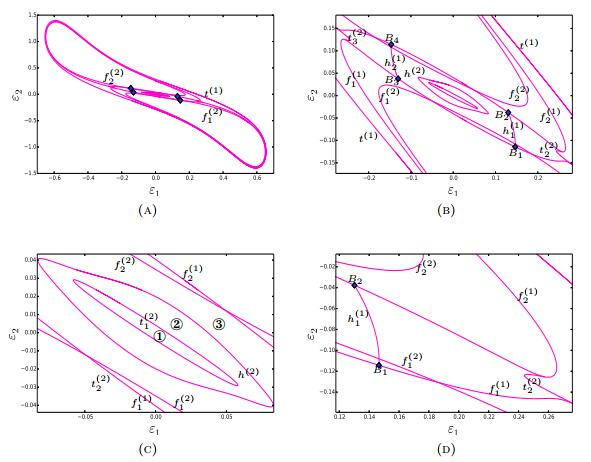
\includegraphics[width=0.85\textwidth]{./modeling_ecology.jpg}
\end{center}
\btVFill
\tiny \vspace{-\baselineskip}\color{berry}{Li et al. 2018, from Gail Wolkowicz's lab at McMaster University}
%My students and I have been formulating and analyzing models motivated by questions in ecology and epidemiology. For example, one goal is to better understand basic population dynamics so that measurable criteria can be developed, enabling scientists to predict combinations of cultures of micro-organisms most effective and safest for use in such processes as water purification and biological waste decomposition. Other applications include pest control, the prevention of species' extinction or the control or eradication of certain diseases. In order to elicit all the potential dynamics, a bifurcation theory approach is used so that the full spectrum of behaviour can be predicted for all appropriate parameter ranges and initial states. Computer simulations are used to elucidate complicated dynamics, to test conjectures, and to reveal properties of the models that are useful in developing analytic proofs. Symbolic computation is used to carry out complicated calculations. The analyses often lead to interesting abstract mathematical problems in dynamical systems, ordinary, integro- and functional differential equations, and bifurcation theory.	
\end{frame}
%%%%%%%%%%%%%%%%%%%%%%%%%%%%%%%%%%%%%%%%%%%%%%%%%%%%%%
%%%%%%%%%%%%%%%%%%%%%%%%%%%%%%%%%%%%%%%%%%%%%%%
\begin{frame}{Broad Types of Bioinformatics}
	\centering
	\Huge
	\begin{enumerate}
		\item \light{Data Analysis
			\item Software Development
		\item Modeling}
	\pause
		\item Combination!
	\end{enumerate}
	
\end{frame}
%%%%%%%%%%%%%%%%%%%%%%%%%%%%%%%%%%%%%%%%%%%%%%%%%%%%%%
%%%%%%%%%%%%%%%%%%%%%%%%%%%%%%%%%%%%%%%%%%%%%%%
\begin{frame}{4. Combination}
\begin{itemize}
	\itm Modelling + Software Development
	\itm Data Analysis + Modelling
	\itm Data Analysis + Software Development
	\itm Data Analysis + Modelling + Software Development
\end{itemize}
\end{frame}
%%%%%%%%%%%%%%%%%%%%%%%%%%%%%%%%%%%%%%%%%%%%%%%%%%%%%%
\begin{frame}{My Research}
	\centering
	\Huge
	\textbf{Spatial Patterns of Molecular Trends in Bacterial Genomes}
	
	\bigskip
	{\normalsize (How do molecular trends change with position in the genome?)}
\end{frame}
%%%%%%%%%%%%%%%%%%%%%%%%%%%%%%%%%%%%%%%%%%%%%%%%%%%%%%%
%%%%%%%%%%%%%%%%%%%%%%%%%%%%%%%%%%%%%%%%%%%%%%%%%%%%%
\begin{frame}{Bacteria are bizarre!}
\textcolor{red}{should I replace this slide with just one crazy pic of HGT?? should I remove this all together? or just shorten it?}
	\pause
	\FourQuad%
	{\centering
		\small{\textbf{H}orizontal \textbf{G}ene \textbf{T}ransfer (\textbf{HGT})}
		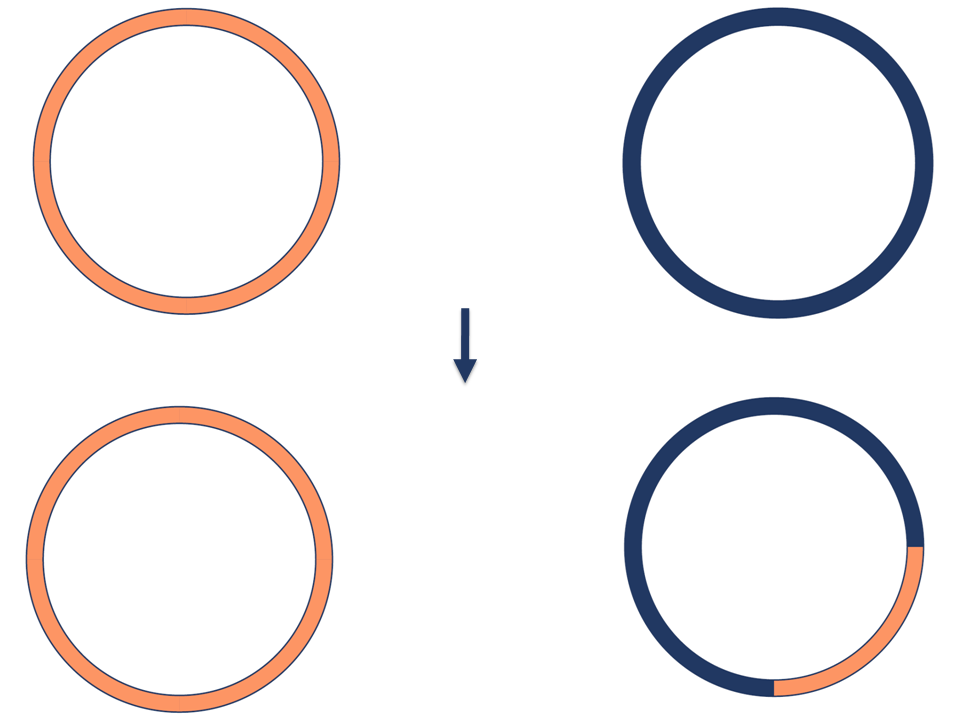
\includegraphics[width=0.75\textwidth]{./bac_genome_reorg_diagrams/HGT_pic.png}}%
	{
	}%
	{
	}%
	{ 
		
	}
\end{frame}


%%%%%%%%%%%%%%%%%%%%%%%%%%%%%%%%%%%%%%%%%%%%%%%%%%%%
\begin{frame}{Bacteria are bizarre!}
	\FourQuad%
	{\centering
		\small{\textbf{H}orizontal \textbf{G}ene \textbf{T}ransfer (\textbf{HGT})}
		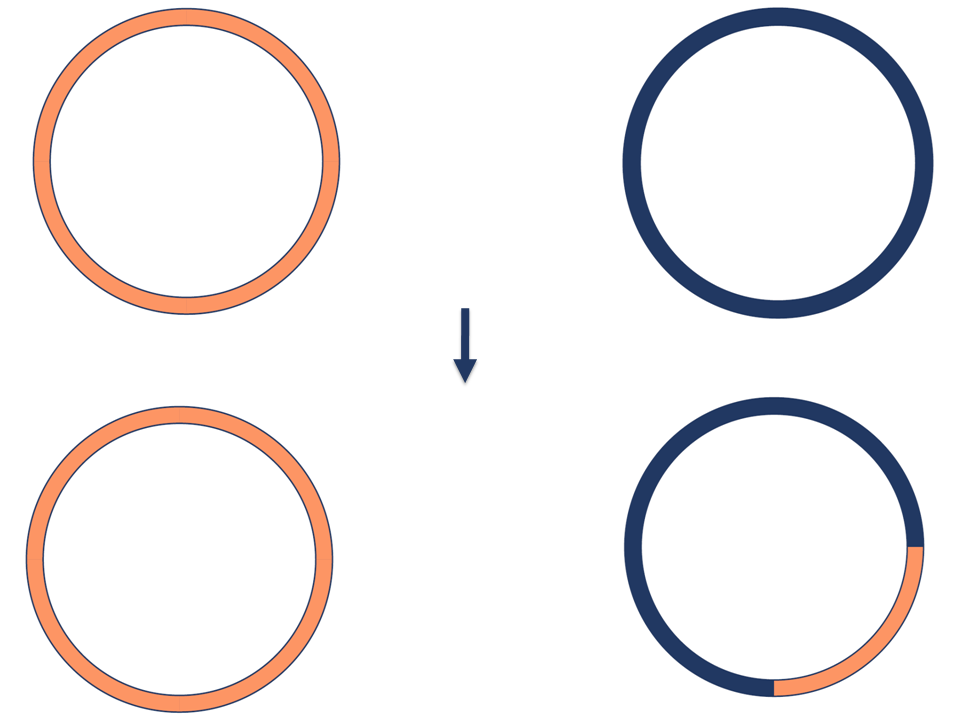
\includegraphics[width=0.75\textwidth]{./bac_genome_reorg_diagrams/HGT_pic.png}}%
	{
	}%
	{ \centering
		\bigskip
		\small{Duplication}
		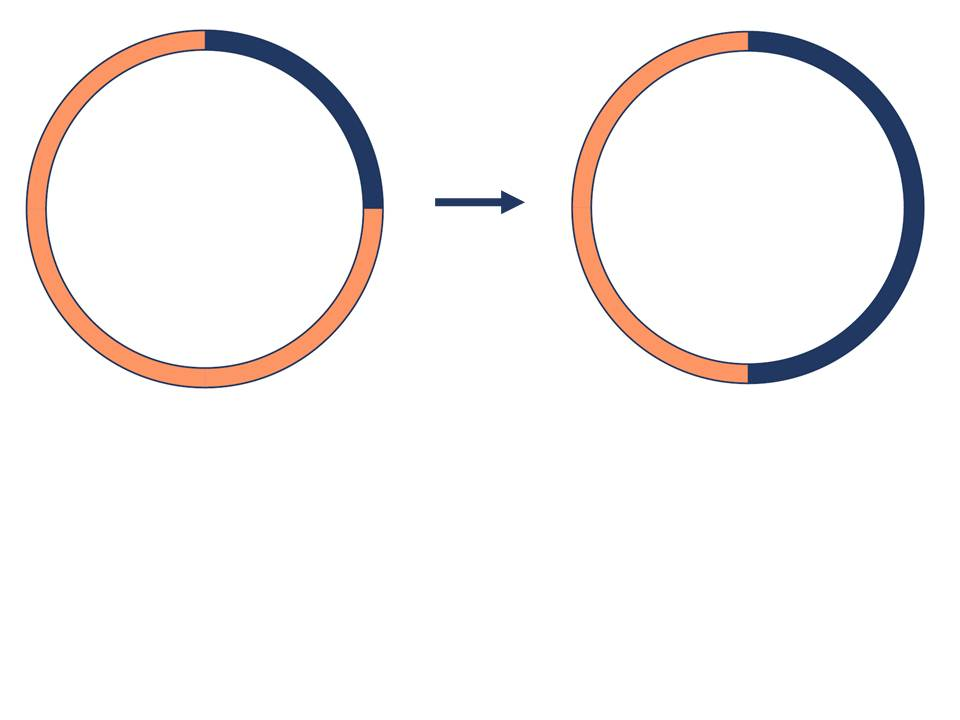
\includegraphics[angle=0, origin=c, width=\textwidth]{./bac_genome_reorg_diagrams/duplication_pic.jpg}
	}%
	{ 
		
	}
\end{frame}

%%%%%%%%%%%%%%%%%%%%%%%%%%%%%%%%%%%%%%%%%%%%%%%%%%%%%
\begin{frame}{Bacteria are bizarre!}
	\FourQuad%
	{\centering
		\small{\textbf{H}orizontal \textbf{G}ene \textbf{T}ransfer (\textbf{HGT})}
		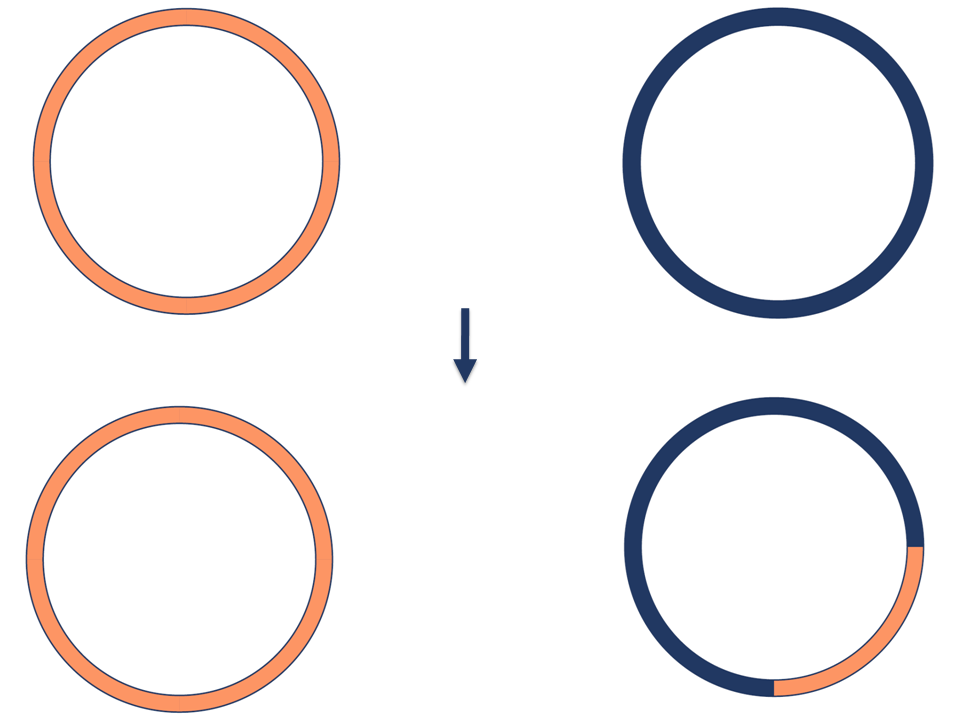
\includegraphics[width=0.75\textwidth]{./bac_genome_reorg_diagrams/HGT_pic.png}}%
	{\centering
		\small{Rearrangement and Translocation}
		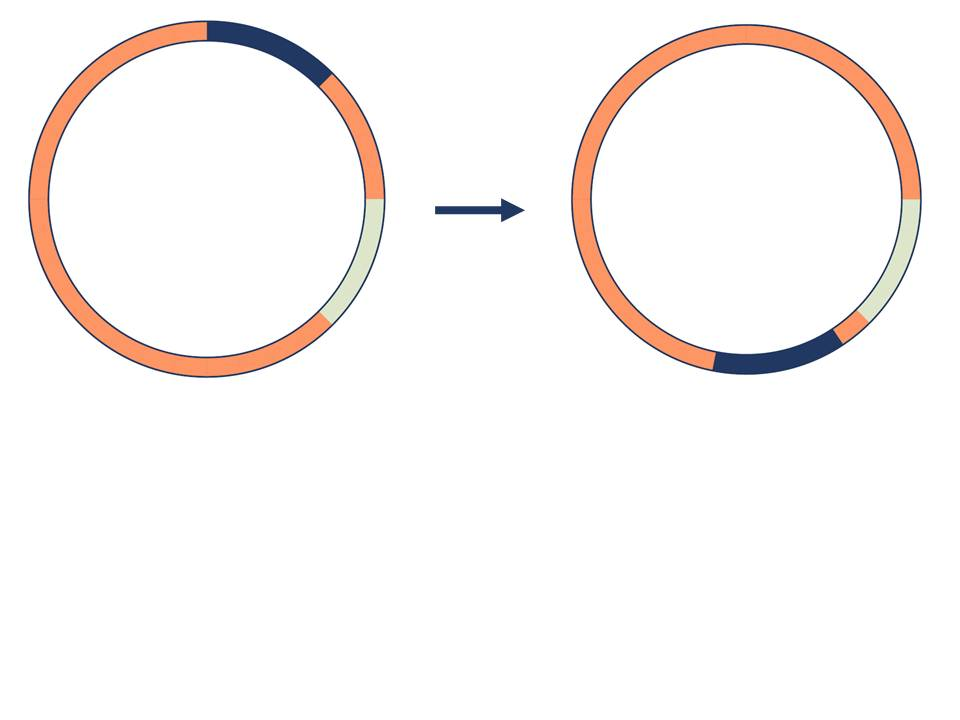
\includegraphics[angle=0, origin=c, width=\textwidth]{./bac_genome_reorg_diagrams/rearrangements_pic.jpg}
	}%
	{ \centering
		\bigskip
		\small{Duplication}
		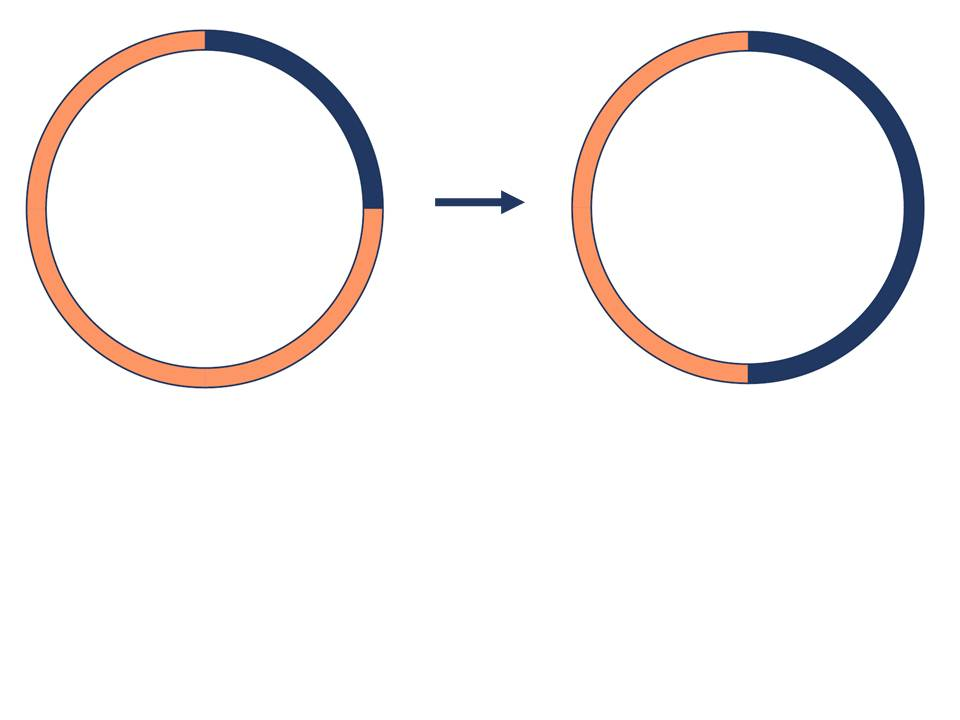
\includegraphics[angle=0, origin=c, width=\textwidth]{./bac_genome_reorg_diagrams/duplication_pic.jpg}
	}%
	{ \centering
		\bigskip
		\small{Inversion}
		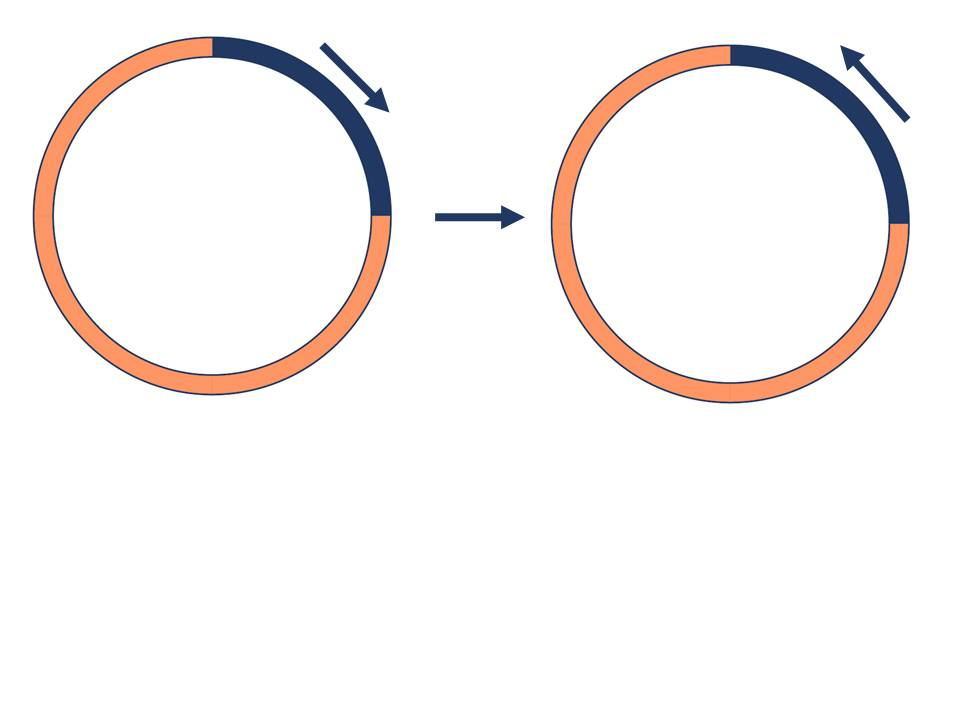
\includegraphics[angle=0, origin=c, width=\textwidth]{./bac_genome_reorg_diagrams/inversion_pic.jpg}
		
	}
\end{frame}
%%%%%%%%%%%%%%%%%%%%%%%%%%%%%%%%%%%%%%%%%%%%%%%%%%%%%
%%%%%%%%%%%%%%%%%%%%%%%%%%%%%%%%%%%%%%%%%%%%%%%%%%%%

\begin{frame}{My Research: Spatial molecular trends}
	\begin{columns}[t]
		\column{.5\textwidth}
		\centering		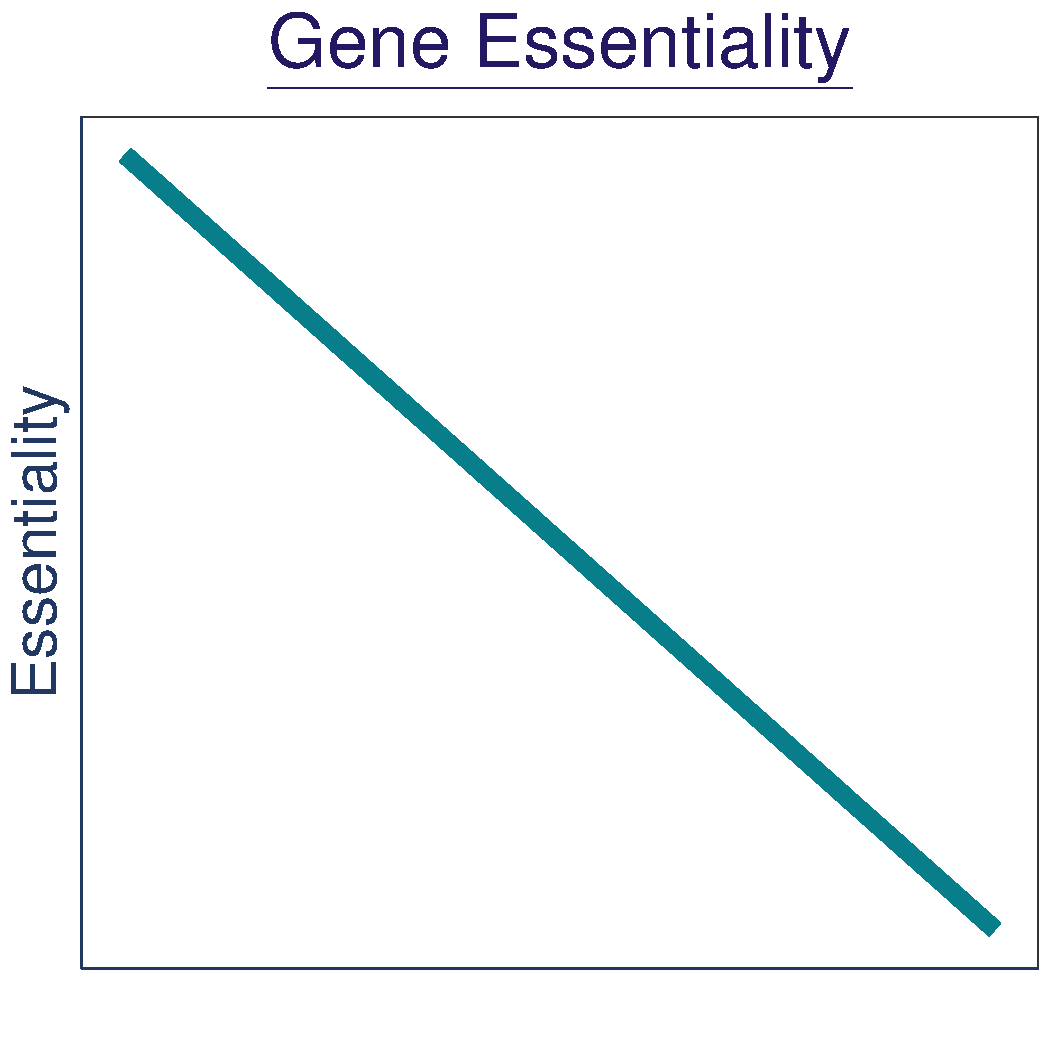
\includegraphics[width=0.67\textwidth]{./Spatial_genome_trends_graphs/ess_graph.pdf}\\
		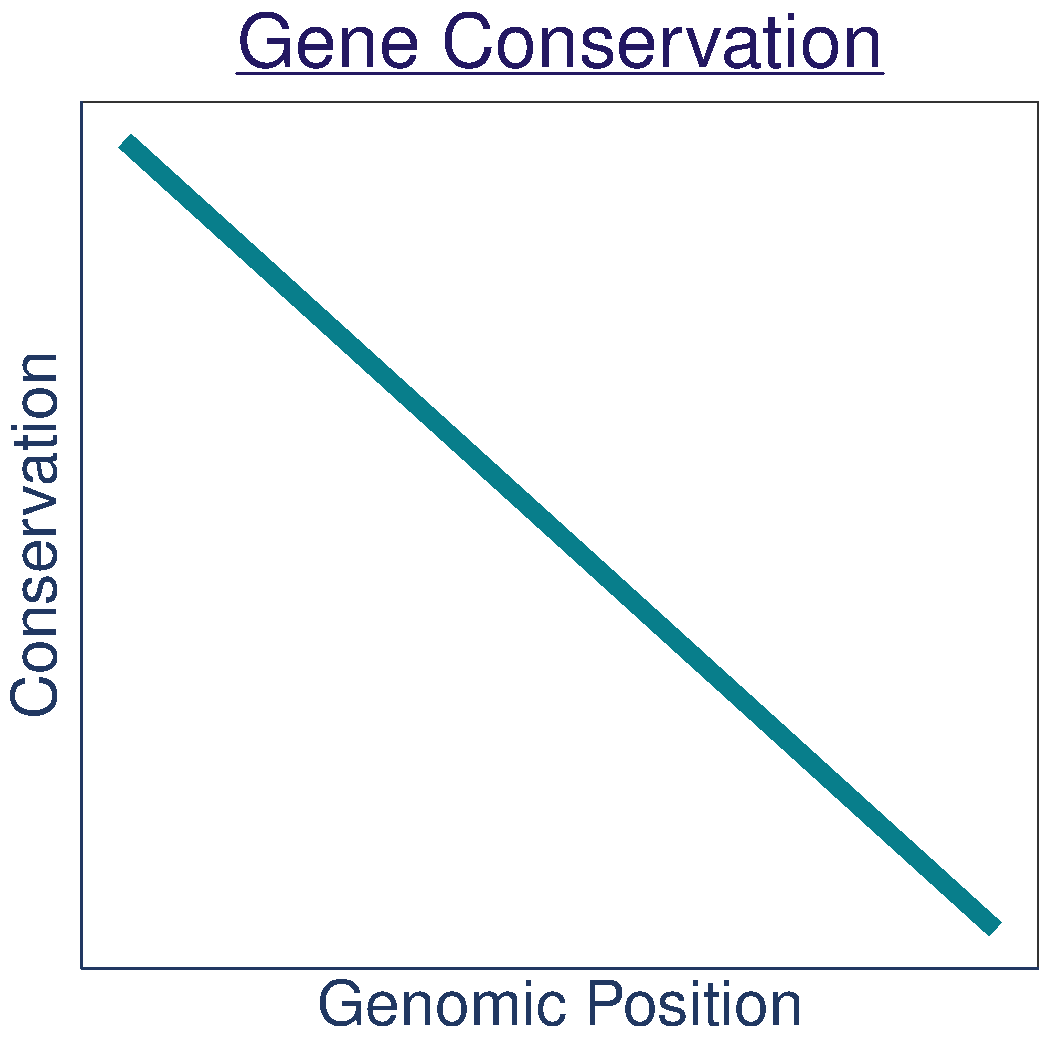
\includegraphics[width=0.67\textwidth]{./Spatial_genome_trends_graphs/cons_graph.pdf}
	
		\column{.5\textwidth}
		\centering	
		\pause		
		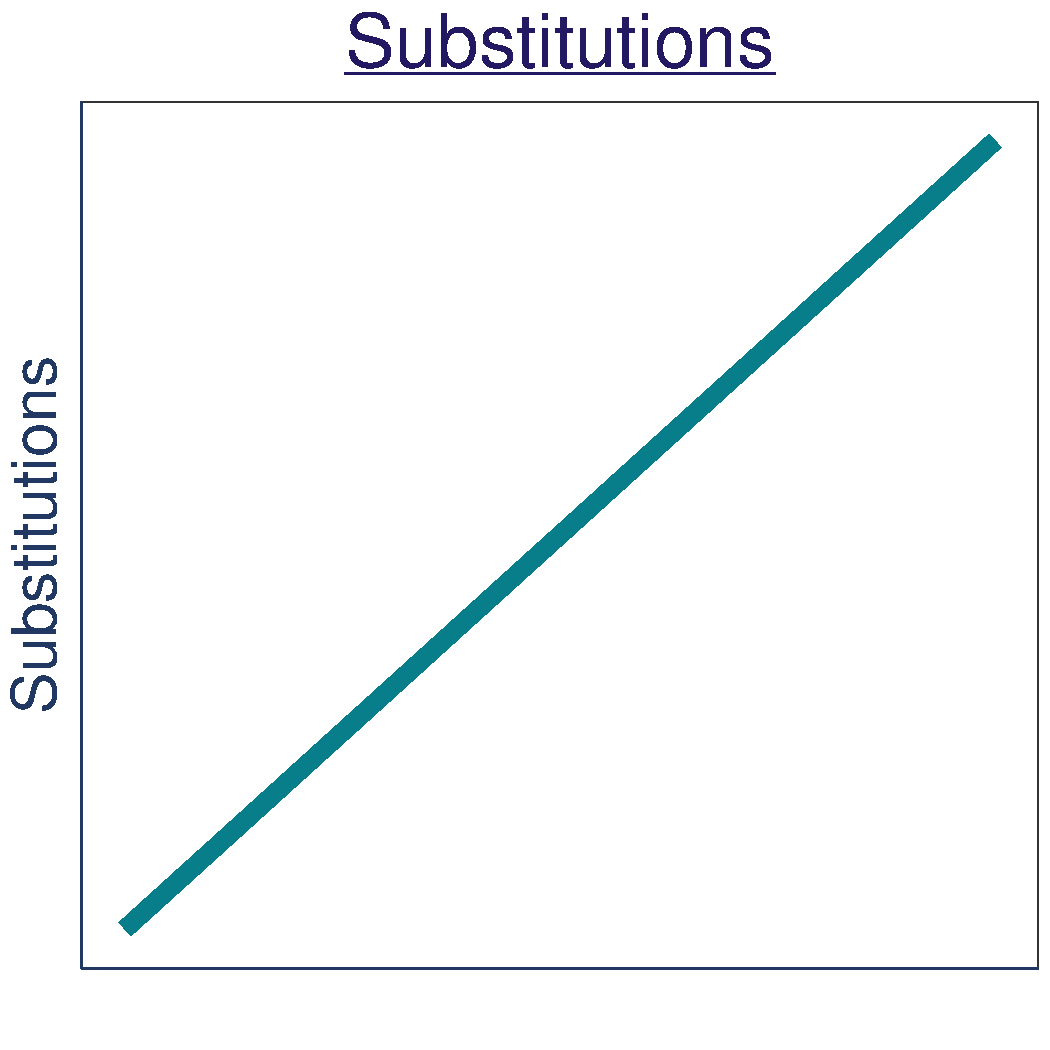
\includegraphics[width=0.67\textwidth]{./Spatial_genome_trends_graphs/mut_graph.pdf}\\
		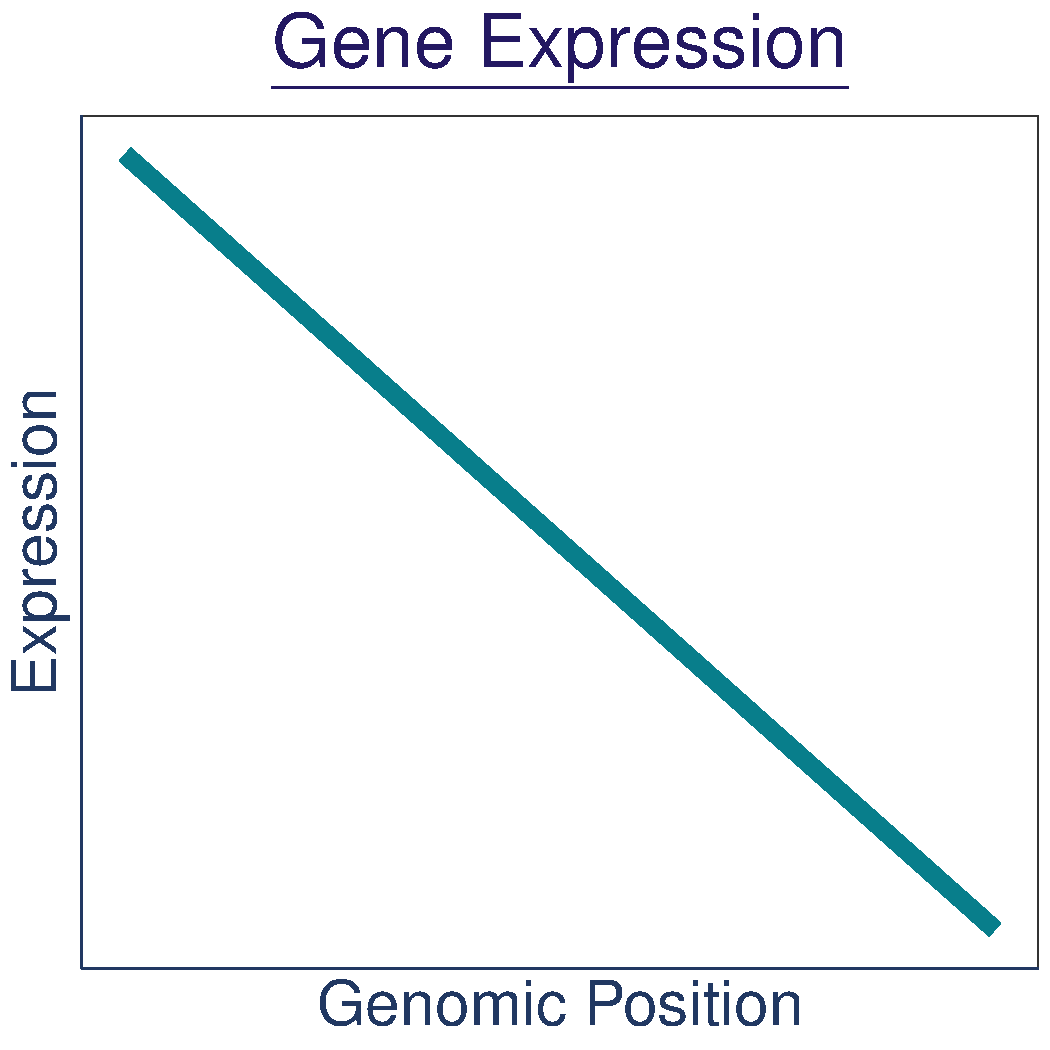
\includegraphics[width=0.67\textwidth]{./Spatial_genome_trends_graphs/exp_graph.pdf}
	\end{columns}
	
	\btVFill
	\tiny \vspace{-\baselineskip}\color{berry}{Couturier et al. 2006, Cooper et al. 2010, Sharp et al. 2005, Morrow et al. 2012, Cooper and Rocha 2006}
	%		\sourceright{Couturier et al. 2006, Cooper et al. 2010, Sharp et al. 2005, Morrow et al. 2012, Cooper and Rocha 2006}
	
\end{frame}
%%%%%%%%%%%%%%%%%%%%%%%%%%%%%%%%%%%%%%%%%%%%%%%%%%%
%%%%%%%%%%%%%%%%%%%%%%%%%%%%%%%%%%%%%%%%%%%%%%%%%%%%

\begin{frame}{My Research: Spatial molecular trends}
	\begin{columns}[t]
		\column{.5\textwidth}
		\centering
%	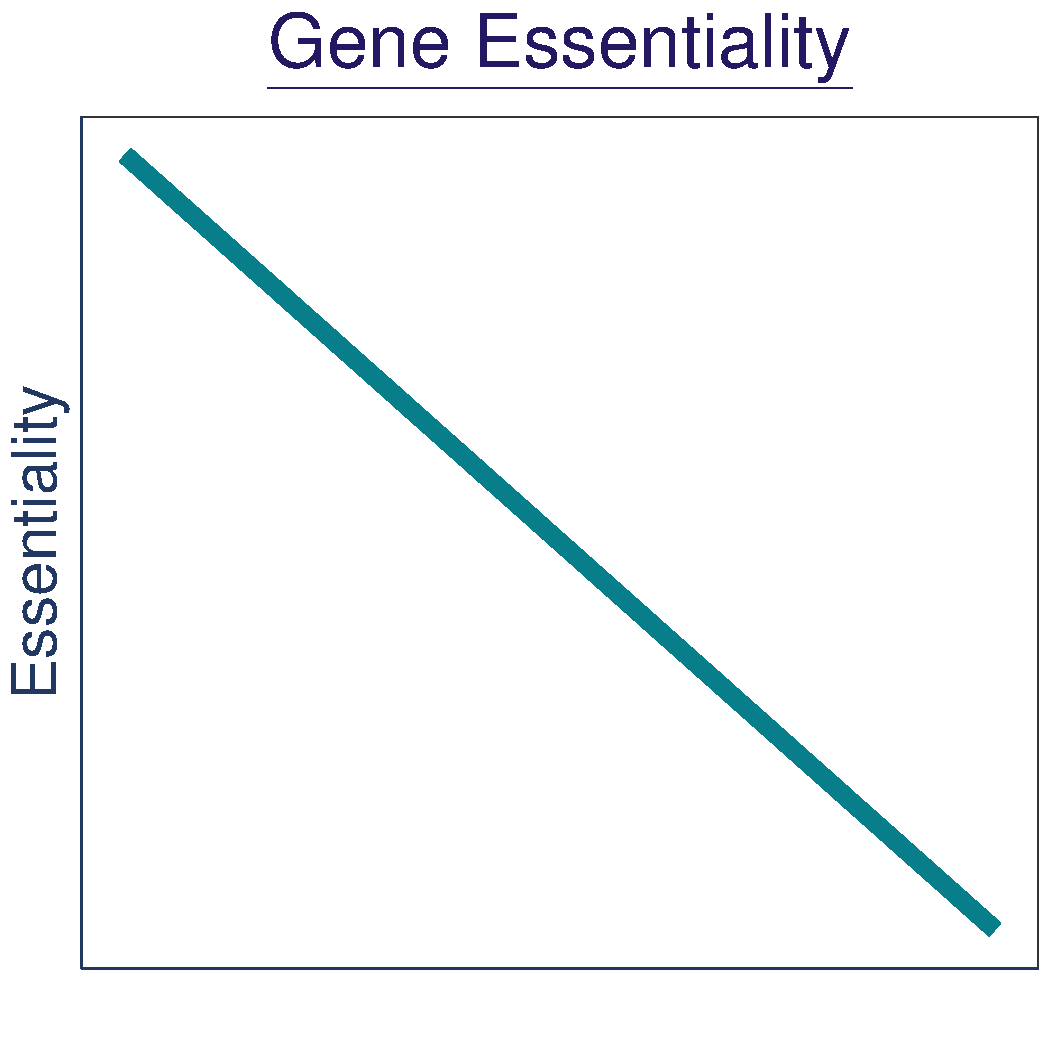
\includegraphics[width=0.67\textwidth]{./Spatial_genome_trends_graphs/ess_graph.pdf}\\
%	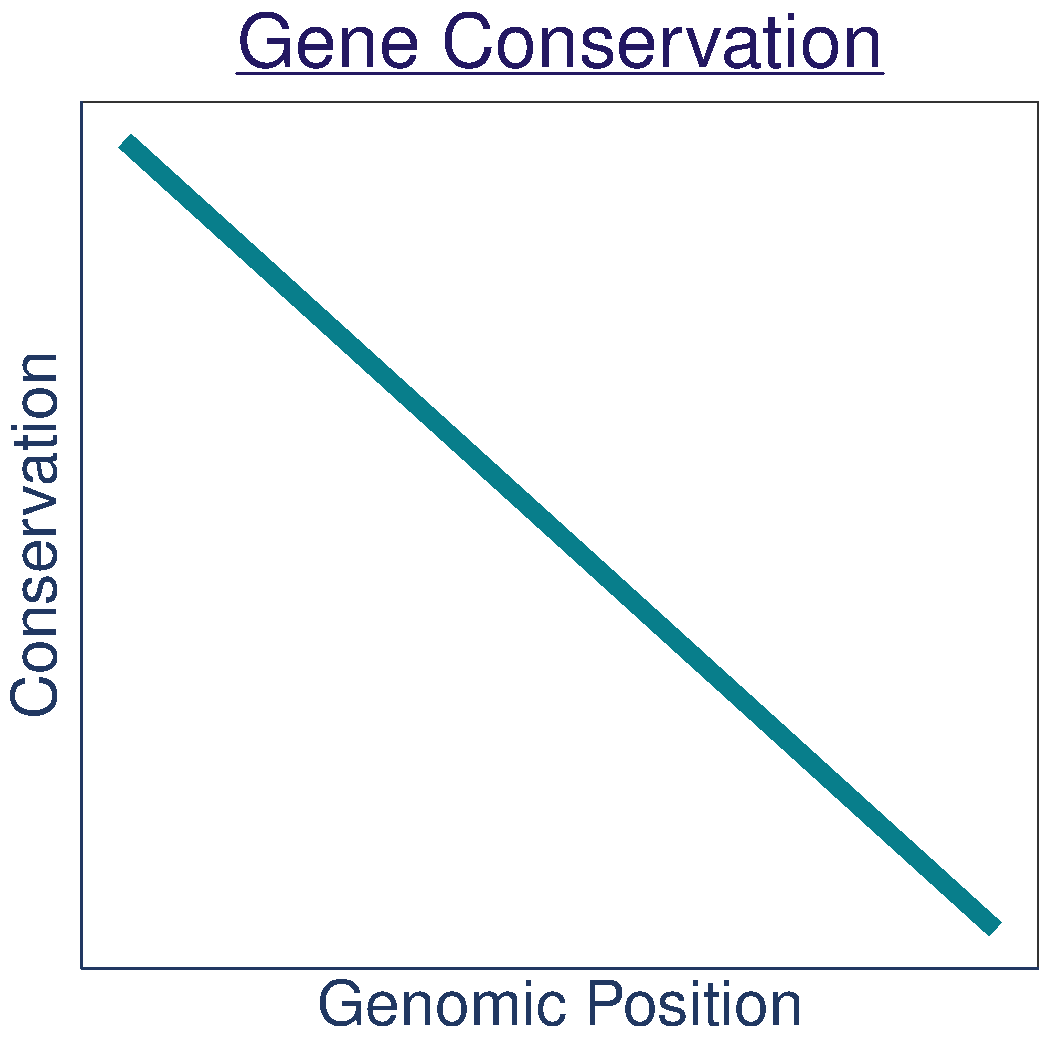
\includegraphics[width=0.67\textwidth]{./Spatial_genome_trends_graphs/cons_graph.pdf}
	
	\column{.5\textwidth}
	\centering	
	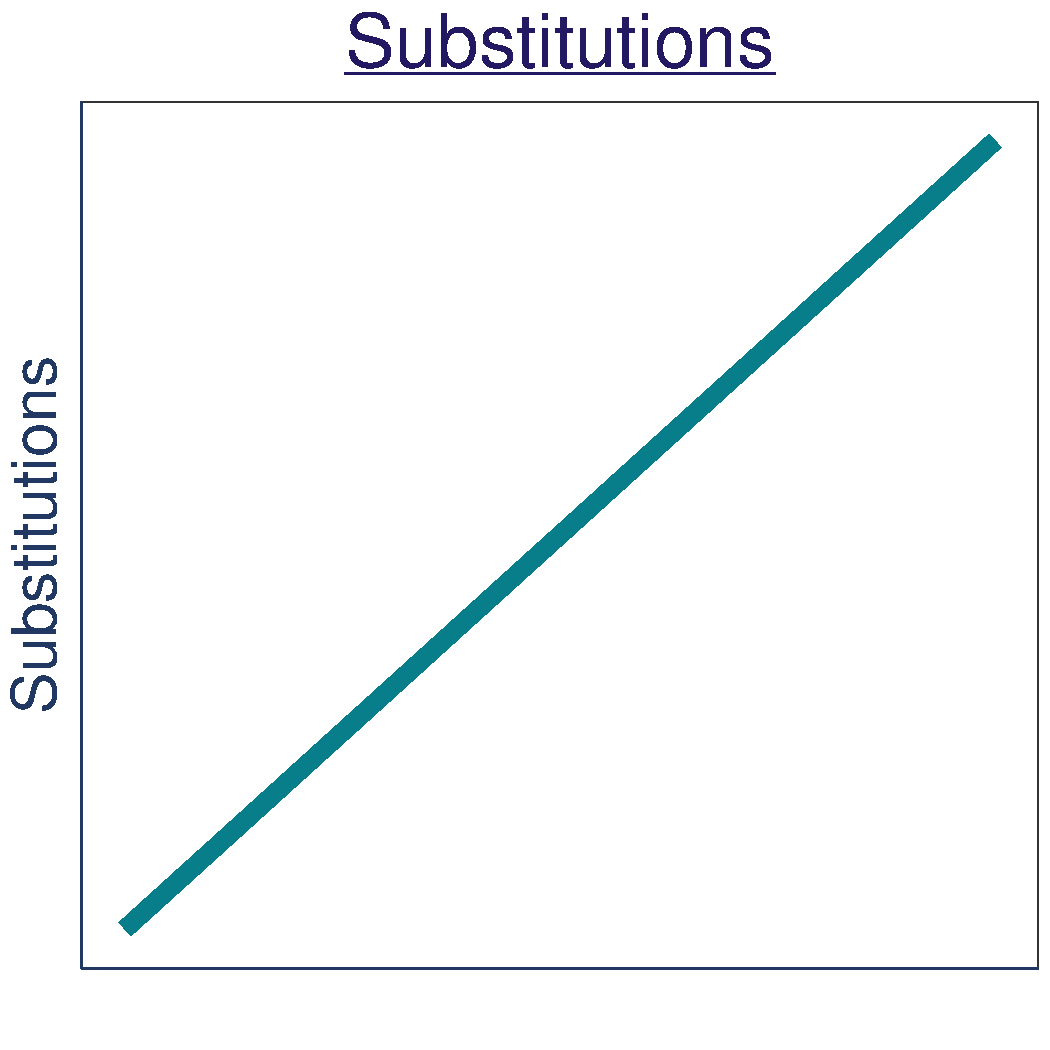
\includegraphics[width=0.67\textwidth]{./Spatial_genome_trends_graphs/mut_graph.pdf}\\
	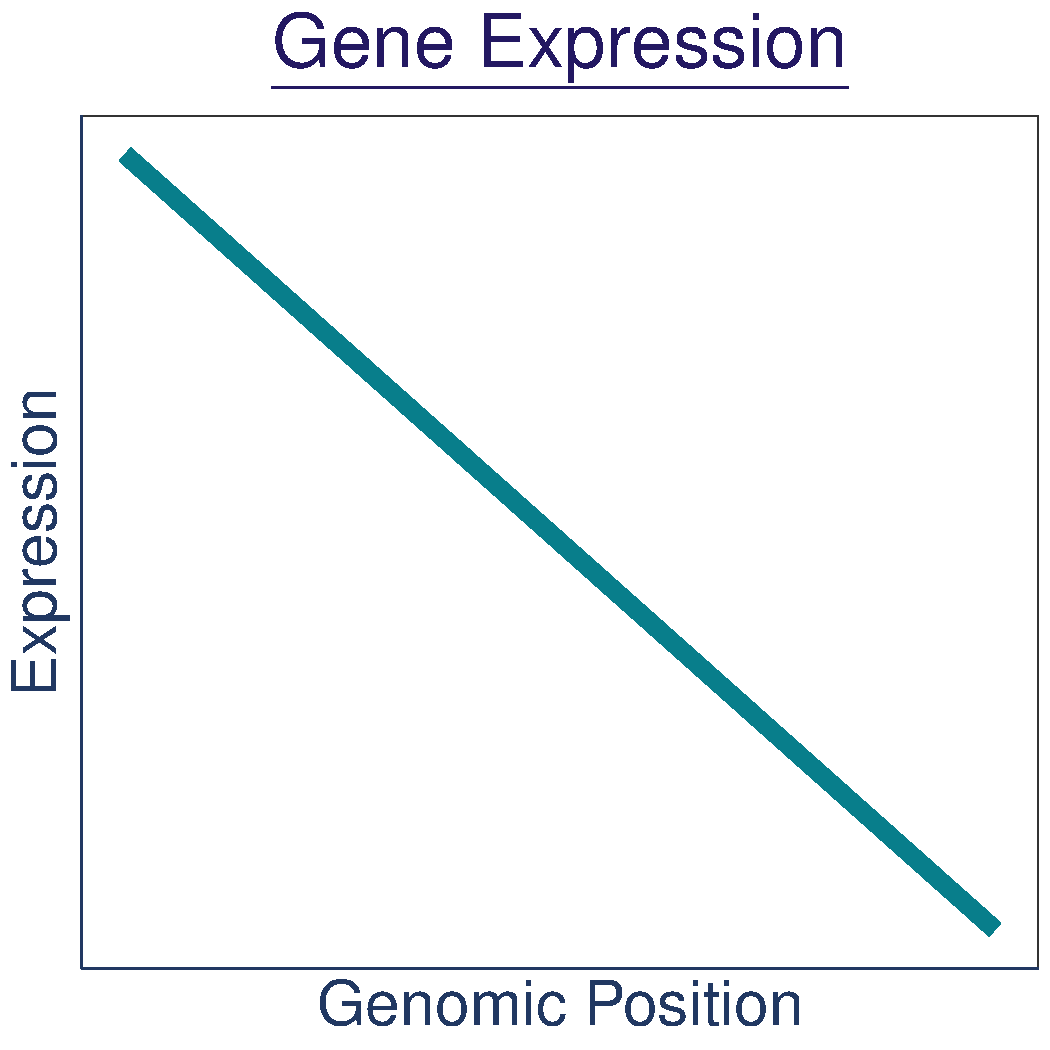
\includegraphics[width=0.67\textwidth]{./Spatial_genome_trends_graphs/exp_graph.pdf}
	\end{columns}
	
	\btVFill
	\tiny \vspace{-\baselineskip}\color{berry}{Couturier et al. 2006, Cooper et al. 2010, Sharp et al. 2005, Morrow et al. 2012, Cooper and Rocha 2006}
	%		\sourceright{Couturier et al. 2006, Cooper et al. 2010, Sharp et al. 2005, Morrow et al. 2012, Cooper and Rocha 2006}
	
\end{frame}
%%%%%%%%%%%%%%%%%%%%%%%%%%%%%%%%%%%%%%%%%%%%%%%
\begin{frame}{My Research: Incorperating Bacteria Genome Shuffling!}
	\begin{center}
		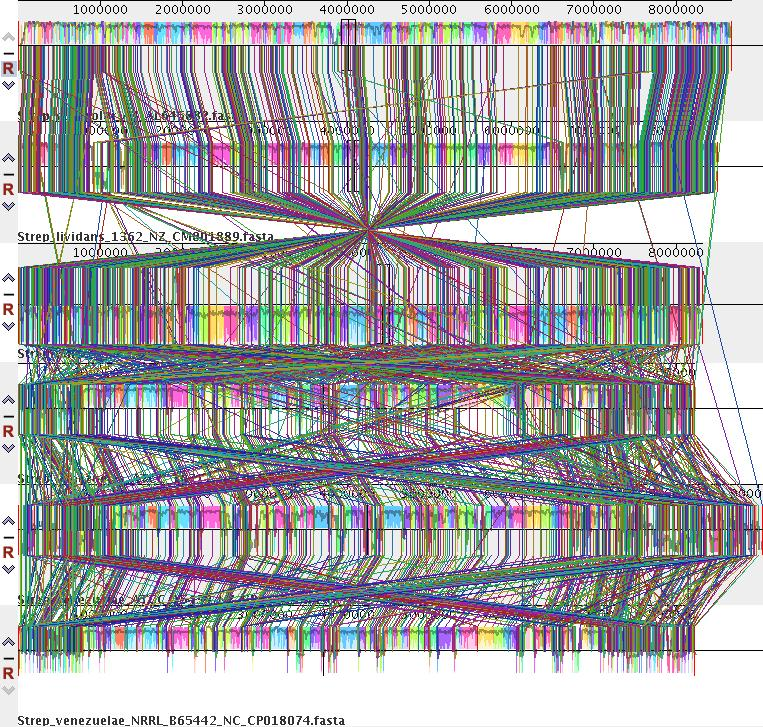
\includegraphics[width=0.8\textwidth]{./figs/6_strep_strains_mauve_aln_pic_13Jan20.jpg}
	\end{center}
%	\btVFill
%	\tiny \vspace{-\baselineskip}\color{berry}{Lato and Golding 2020, Under Review }
\end{frame}
%%%%%%%%%%%%%%%%%%%%%%%%%%%%%%%%%%%%%%%%%%%%%%%%%%%%%%
%%%%%%%%%%%%%%%%%%%%%%%%%%%%%%%%%%%%%%%%%%%%%%%%%%%
\begin{frame}{My Research: The Organisms}
	Bacteria:
	\bi
	\itm \ecoli
	\itm \bas
	\itm \strep
	\itm \sm
	\ei
	\vfill
	
	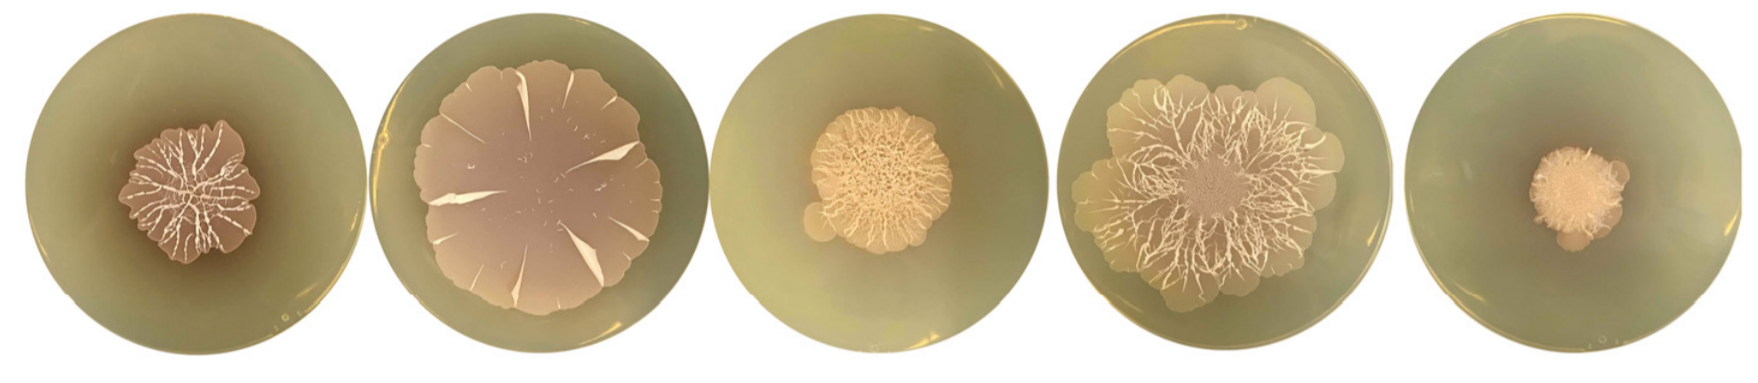
\includegraphics[width=\textwidth]{strep_pic}
	%\begin{figure}
	%	\hfill\begin{minipage}{.5\textwidth}\centering
	%		\includegraphics[scale=0.4]{smel_pic}
	%		
	\centering
	{\centering \tiny\textcolor{berry}{ Photo: \strep by Stephanie Jones, Marie Elliot's Lab at McMaster University}}
	%		%		\caption{\texttt{minipage}}
	%	\end{minipage}
	%\end{figure}
\end{frame}
%%%%%%%%%%%%%%%%%%%%%%%%%%%%%%%%%%%%%%%%%%%%%%%%%%%%
%%%%%%%%%%%%%%%%%%%%%%%%%%%%%%%%%%%%%%%%%%%%%%%%%%
\begin{frame}{My Research: Conclusions}
	\begin{columns}[t]
		\column{.5\textwidth}
		\centering
		\textbf{Previous Studies:} 
		
		\bigskip
		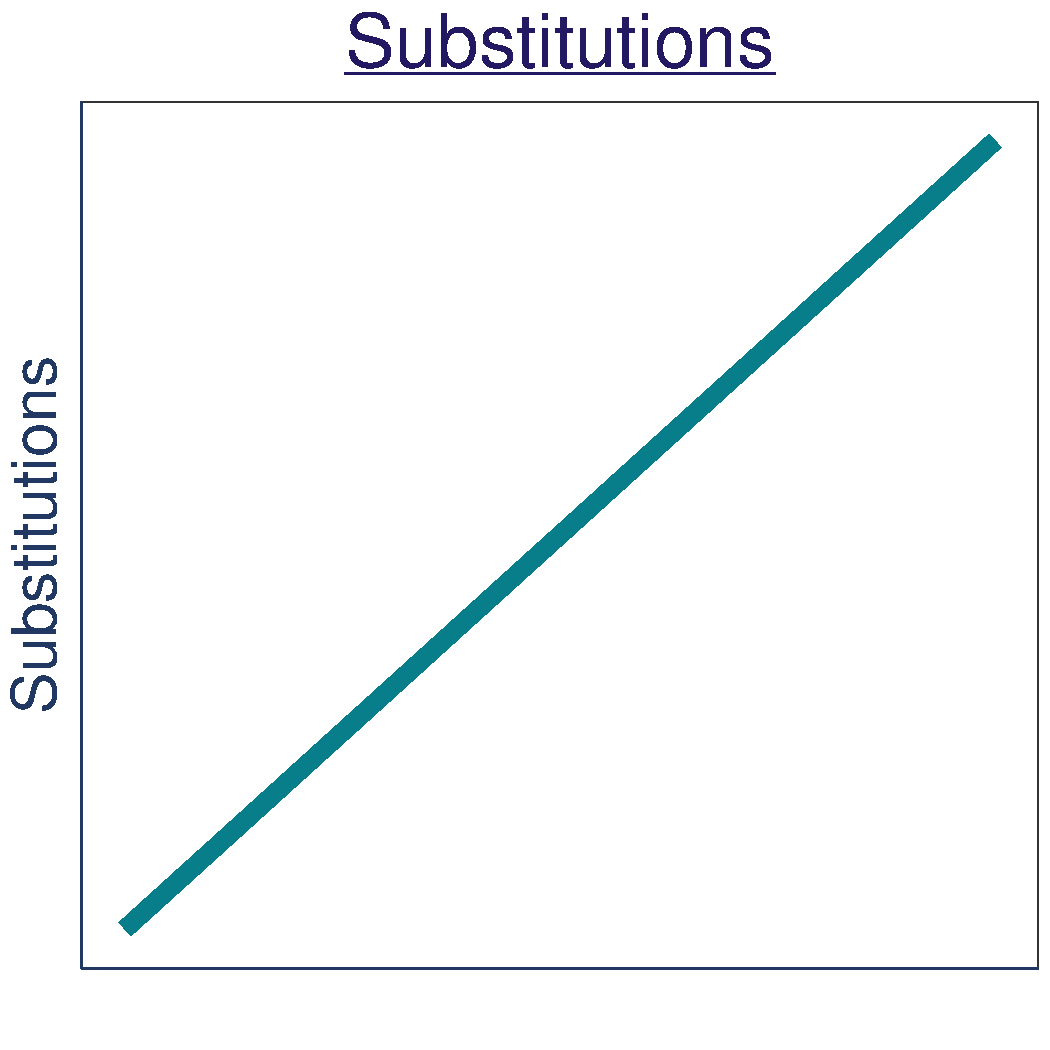
\includegraphics[width=0.65\textwidth]{./Spatial_genome_trends_graphs/mut_graph.pdf}\\
		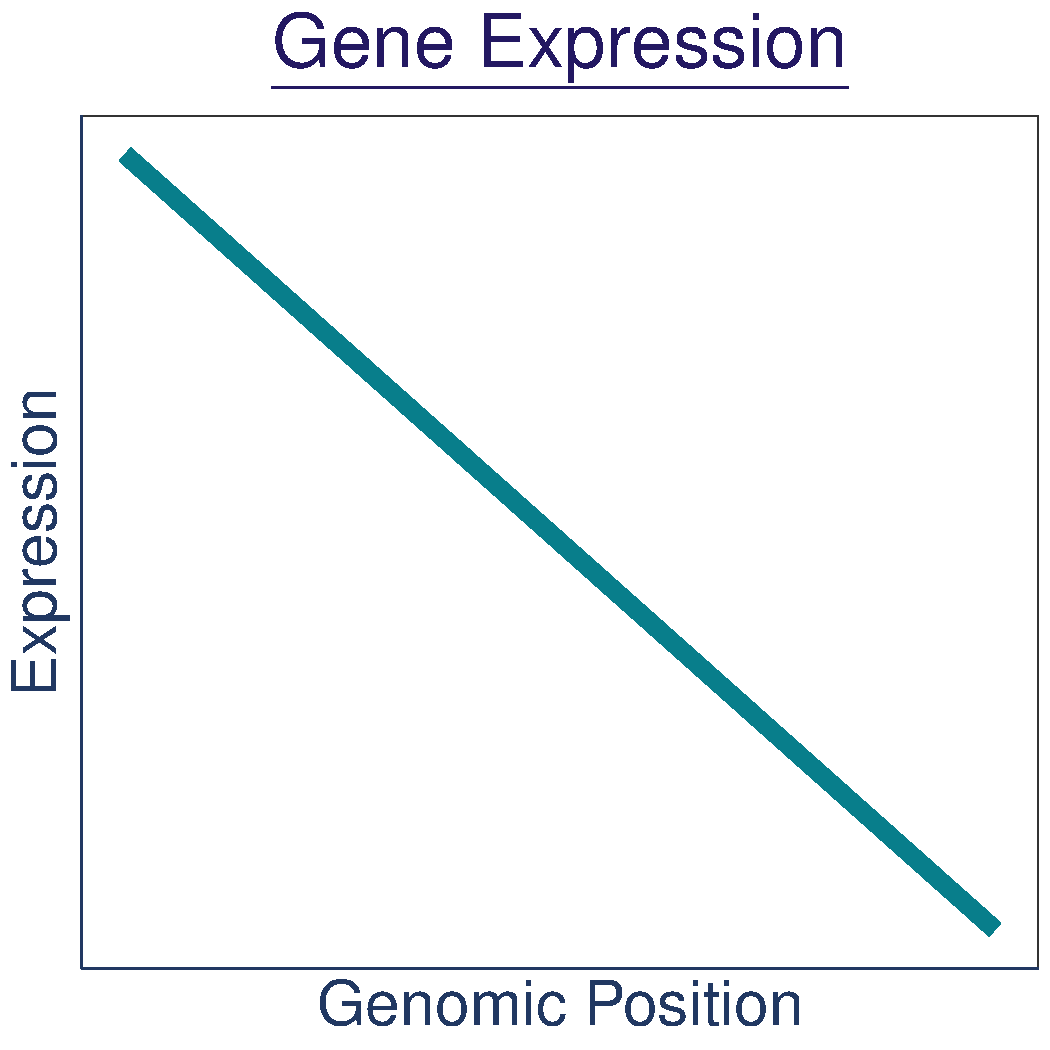
\includegraphics[width=0.65\textwidth]{./Spatial_genome_trends_graphs/exp_graph.pdf}
		\column{.5\textwidth}
		\pause
		\centering
		\textbf{My Research:}
		
		\bigskip
		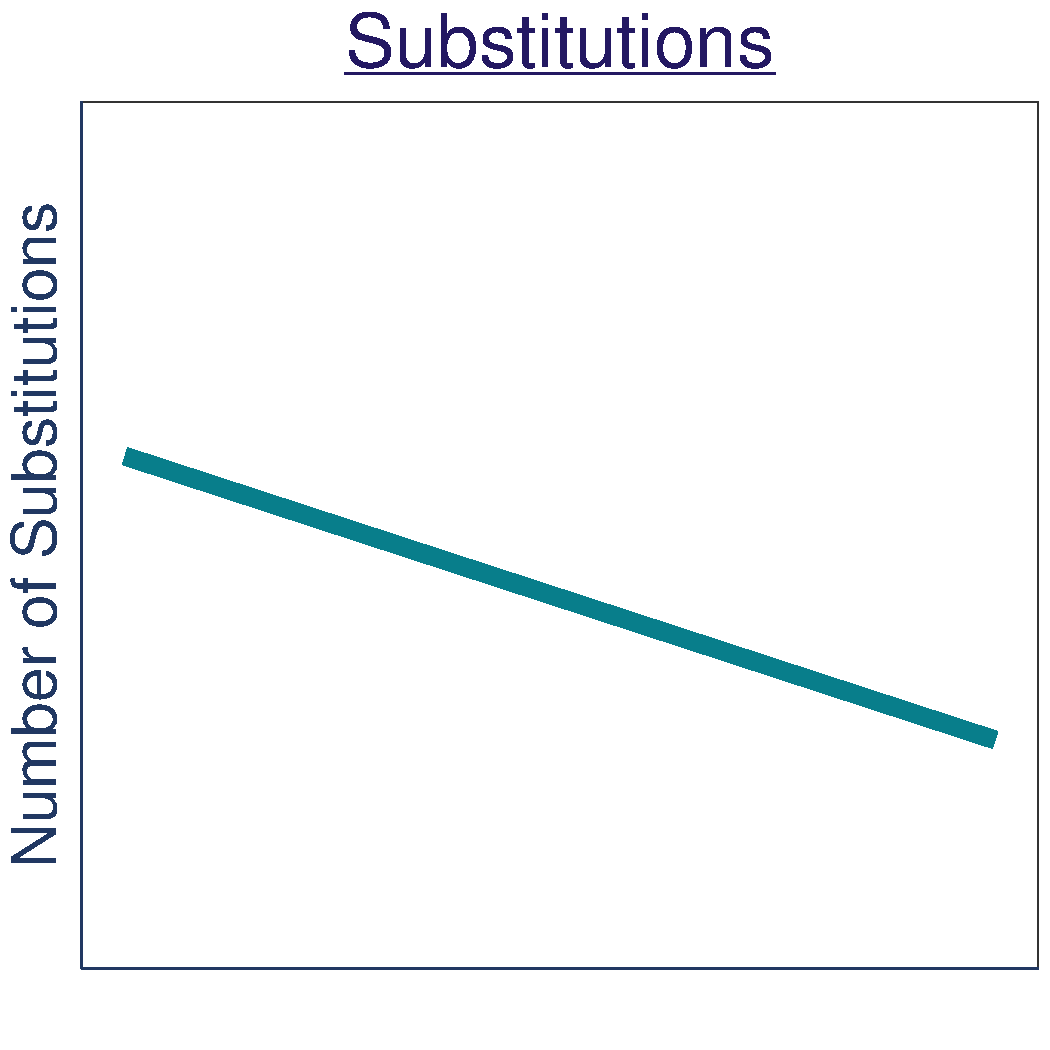
\includegraphics[width=0.65\textwidth]{./Spatial_genome_trends_graphs/sub_results_graph.pdf}\\
		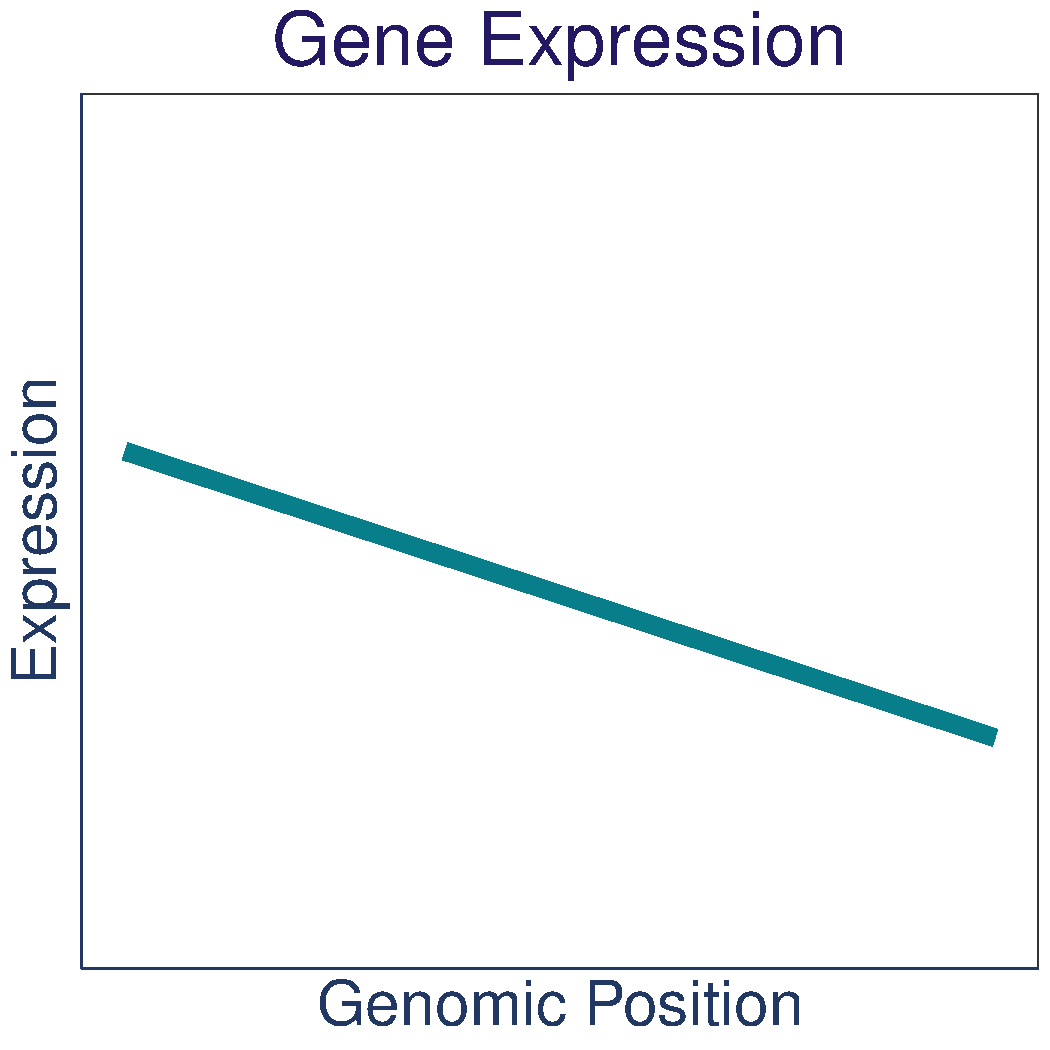
\includegraphics[width=0.65\textwidth]{./Spatial_genome_trends_graphs/exp_results_graph.pdf}
	\end{columns}
\end{frame}
%%%%%%%%%%%%%%%%%%%%%%%%%%%%%%%%%%%%%%%%%%%%%%%%%%
%%%%%%%%%%%%%%%%%%%%%%%%%%%%%%%%%%%%%%%%%%%%%%%
\begin{frame}{Why become a Comp Bio Geek?}
	\centering
	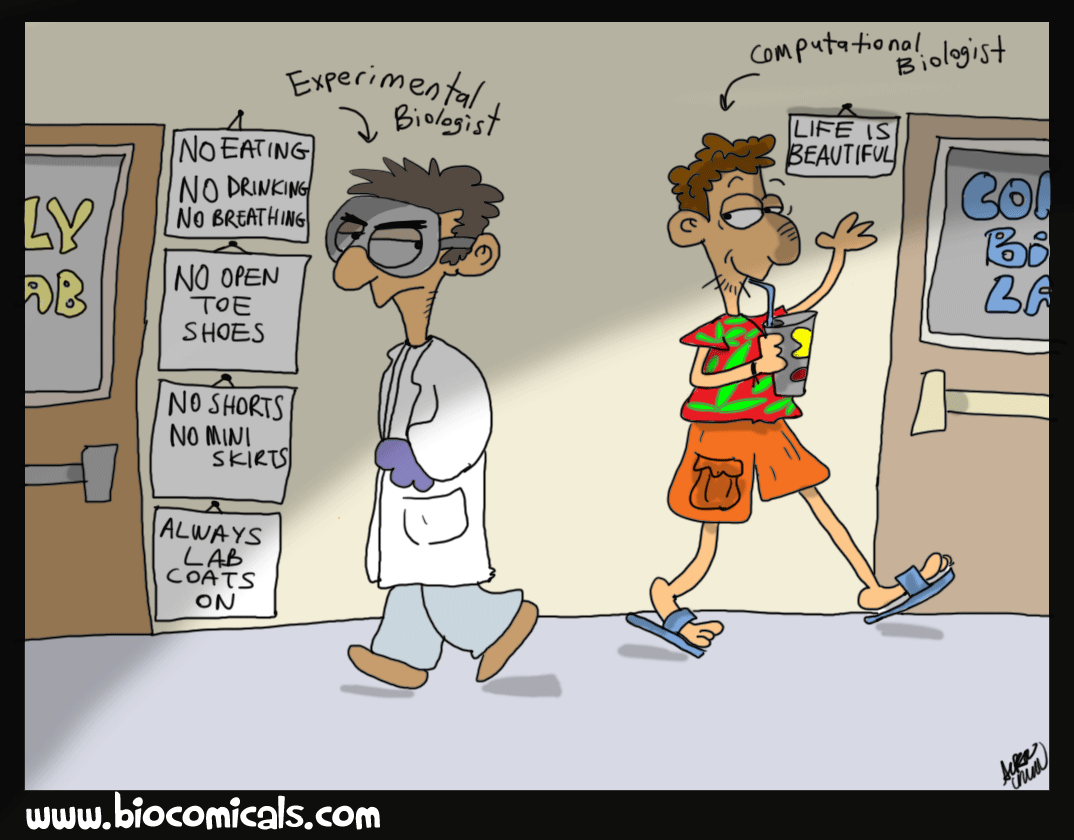
\includegraphics[width=0.95\textwidth]{./comp_bio.png}
	
\end{frame}
%%%%%%%%%%%%%%%%%%%%%%%%%%%%%%%%%%%%%%%%%%%%%%%%%%%%%%
%%%%%%%%%%%%%%%%%%%%%%%%%%%%%%%%%%%%%%%%%%%%%%%
\begin{frame}{Not Just Biology!}
			\begin{columns}[t]
			\column{.5\textwidth}
			\centering
			\pause
		%	\bigskip
				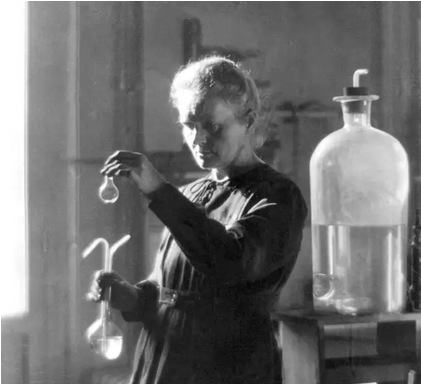
\includegraphics[width=0.7\textwidth]{./figs/marie_curie.png}
			
			{\tiny \textcolor{berry}{Marie Curie, Nobel Prize in Chemistry}}\\
			\pause
			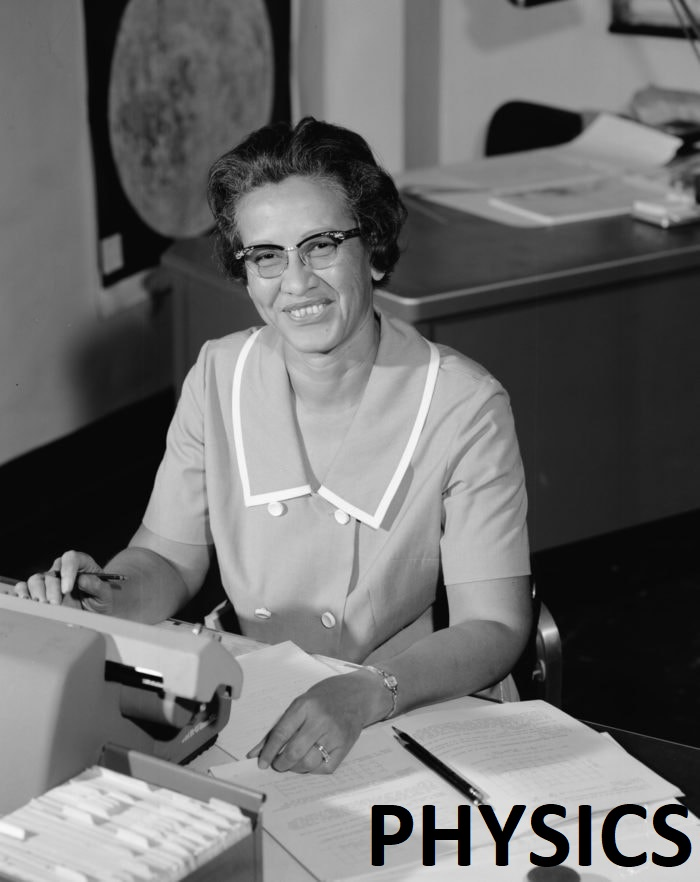
\includegraphics[width=0.55\textwidth]{./figs/katherine_johnson.jpg}
			
			{\tiny \textcolor{berry}{Katherine Johnson, NASA Physicist}}
			\column{.5\textwidth}
			\pause
			\centering
			\bigskip
			
\includegraphics[width=0.65\textwidth]{./figs/fb.png}\\
			
\includegraphics[width=0.65\textwidth]{./figs/insta.png}
		\end{columns}
	
\end{frame}
%%%%%%%%%%%%%%%%%%%%%%%%%%%%%%%%%%%%%%%%%%%%%%%
\begin{frame}{Courses you should take or audit:}
	\LARGE
	\begin{itemize}
		\itm \textbf{Online Resources!}
		\begin{itemize}
			\itm \texttt{DataCamp}, \texttt{Coursera}, \texttt{Codeacademy}
		\end{itemize}
		\itm \textbf{Bio 3S03:} Intro to Bioinformatics  \sloppy
		\itm \textbf{Bio 3SS3:} Population Ecology
		\itm \textbf{Bio 3SA3:} Applied Statistics for Biology
		\itm \textbf{Math 4MB3:} Mathematical Biology
		\itm \textbf{Math 3MB3:} Introduction to Modelling
		 
	\end{itemize}
	
\end{frame}
%%%%%%%%%%%%%%%%%%%%%%%%%%%%%%%%%%%%%%%%%%%%%%%
\begin{frame}{}
\begin{center}
	\Huge
	
	\bigskip
	
	\textbf{Questions?}
	
	\bigskip
	
	\Large latodf@mcmaster.ca
	
	\bigskip
	\centering
	
\includegraphics[width=0.3\textwidth]{./figs/qr_code.pdf}
\end{center}
	
\end{frame}
\end{document}
